\documentclass[11pt,a4paper]{report}
\usepackage[utf8]{inputenc}
\usepackage{amsmath,amssymb,amsfonts,amsthm}
\usepackage{mathtools}
\usepackage{booktabs}
\usepackage{graphicx}
\usepackage{hyperref}
\usepackage{cleveref}
\usepackage{geometry}
\usepackage{listings}
\usepackage{tikz}
\usepackage{xcolor}
\usepackage{microtype}
\usepackage{algorithm}
\usepackage{algpseudocode}
\usepackage{tabularx}
\usepackage{longtable}

\newtheorem{theorem}{Theorem}
\newtheorem{corollary}{Corollary}[theorem]

\geometry{
  a4paper,
  left=25mm,
  right=25mm,
  top=25mm,
  bottom=25mm
}

\hypersetup{
    colorlinks=true,
    linkcolor=blue,
    filecolor=magenta,      
    urlcolor=cyan,
    pdftitle={Socrates in the Loop: Optimising Multi-Agent Tutoring Systems via Cognitive Epistemic Simulation},
    pdfpagemode=UseNone,
    plainpages=false,
    hypertexnames=false,
}

% Code listing setup
\definecolor{codegreen}{rgb}{0,0.6,0}
\definecolor{codegray}{rgb}{0.5,0.5,0.5}
\definecolor{codepurple}{rgb}{0.58,0,0.82}
\definecolor{backcolour}{rgb}{0.96,0.96,0.96}

\lstdefinestyle{pythonstyle}{
    backgroundcolor=\color{backcolour},   
    commentstyle=\color{codegreen},
    keywordstyle=\color{blue}\bfseries,
    numberstyle=\tiny\color{codegray},
    stringstyle=\color{codepurple},
    basicstyle=\ttfamily\footnotesize,
    breakatwhitespace=false,         
    breaklines=true,                 
    captionpos=b,                    
    keepspaces=true,                 
    numbers=left,                    
    numbersep=5pt,                  
    showspaces=false,                
    showstringspaces=false,
    showtabs=false,                  
    tabsize=4
}
\lstset{style=pythonstyle}

% TikZ configurations
\usetikzlibrary{shapes.geometric, arrows, positioning, fit, calc}
\tikzstyle{startstop} = [draw, rectangle, rounded corners, minimum width=3cm, minimum height=1cm,text width=3cm, text centered, draw=blue!50, fill=blue!10]
\tikzstyle{process} = [draw, rectangle, minimum width=3cm, minimum height=1cm, text width=3cm, text centered, draw=orange!50, fill=orange!10]
\tikzstyle{decision} = [draw, diamond, aspect=2, minimum width=3cm, minimum height=1cm, text width=2.5cm, text centered, draw=green!50, fill=green!10]
\tikzstyle{arrow} = [thick,->,>=stealth]

\newcolumntype{Y}{>{\raggedright\arraybackslash}X}
\newcolumntype{P}[1]{>{\raggedright\arraybackslash}p{#1}}
\setlength{\LTpre}{0.5\baselineskip}
\setlength{\LTpost}{0.5\baselineskip}

\begin{document}

% --- TITLE PAGE ---
\begin{titlepage}
    \centering
    \vspace*{2cm}
    {\Huge \bfseries Socrates in the Loop: \\ Optimising Multi-Agent Tutoring Systems via Cognitive Epistemic Simulation \par}
    \vspace{1.5cm}
    {\Large \bfseries MSc Computing (Artificial Intelligence \& Machine Learning) \par}
    \vspace{0.5cm}
    {\large Department of Computing, Imperial College London \par}
    \vspace{2cm}
    {\large \textbf{Student Candidate:} Anas Khan \par}
    {\large \textbf{Date:} May 2026 \par}
    \vspace{2cm}
    {\large \textbf{Academic Advisors:} \par}
    {\large Department of Computing Faculty Panel \par}
    \vfill
    {\large Imperial College London \par}
\end{titlepage}

% --- FRONT MATTER ---
\pagenumbering{roman}

\begin{abstract}
Large Language Models (LLMs) have become powerful tools for information retrieval, yet their default optimisation towards direct answer generation bypasses the cognitive struggle essential for durable human learning. This dissertation presents the design and implementation of a Socratic Multi-Agent System (MAS) for computer science education, built to guide students towards conceptual mastery through adaptive Socratic questioning. Evaluating such systems with live human cohorts carries substantial financial, ethical, and operational costs at the prototype stage. To support early-stage design without over-claiming human efficacy, we propose an Agent-in-the-Loop Epistemic Simulation: a controlled simulation environment for stress-testing tutor policies against cognitively constrained student agents before any human deployment. We address three structural limitations in current educational agent simulation: (1) Cognitive Bandwidth and Friction Modelling (CBFM), which operationalises prompt complexity, working-memory pressure, and Zone of Proximal Development mismatch as explicit simulator variables; (2) Sycophancy Mitigation via Adversarial Scratchpad Probing, which reduces dialogue-level agreement bias by separating public student utterances from independent diagnostic code execution; and (3) POMDP Tutor Policy Evaluation, which compares offline Q-learning over interpretable Socratic directives against strong heuristic and contextual-bandit alternatives. A cyclic multi-agent graph in LangGraph orchestrates the Socratic tutor, epistemic tracker, and pedagogical guardrail, with simulated learning gains triangulated through held-out diagnostic probes, leakage measurements, ablation studies, and expert transcript ratings.
\end{abstract}

\newpage
\tableofcontents
\newpage

% --- MAIN MATTER ---
\pagenumbering{arabic}

\chapter{Introduction}
\label{ch:intro}

\section{Context and Educational Grounding}
When a student asks an AI assistant to write a sorting algorithm, receives working code, submits it, and earns full marks, yet cannot explain why the loop terminates when asked one week later, a fundamental educational failure has occurred. This failure is not incidental; it is structural. AI dialogue systems optimise for fluency and helpfulness, systematically bypassing the cognitive struggle that produces durable understanding \cite{bjork1994memory}. The very ease with which a student obtains a correct answer is the mechanism by which deep learning is short-circuited.

Cognitive science identifies this as the consequence of bypassing \textit{desirable difficulties} \cite{bjork1994memory}: the productive friction of retrieval practice, effortful schema construction, and self-explanation that consolidates knowledge from working memory into long-term storage \cite{roediger2006test}. Providing a direct answer eliminates this friction entirely, leaving the student with surface familiarity rather than transferable expertise. In programming education, where abstract concepts must be applied flexibly to novel problems, this distinction is decisive.

Socratic tutoring addresses this directly. Rather than supplying answers, a Socratic tutor strategically withholds them, asking guided diagnostic questions, surfacing misconceptions, and scaffolding the learner towards independent discovery. The critical technical challenge is that a student's true knowledge state is hidden: a tutor cannot read what a learner genuinely understands from their conversational responses alone. What a student \textit{says} they know and what they \textit{actually} know are two distinct signals, and conflating them — as all current LLM tutors do — produces fundamentally unreliable educational evaluations, a vulnerability we address via Adversarial Scratchpad Probing (Section~2.4.4).

This hidden-state problem motivates a probabilistic approach to tutoring. Because the tutor cannot directly inspect what a learner understands, the system must maintain a running probability distribution over plausible student knowledge states, updating it at every dialogue turn. We formalise this as a Partially Observable Markov Decision Process (POMDP) (Section~2.4.1), in which a dedicated \textit{Epistemic Tracker} infers the student's hidden state (Section~2.4.2) and a constrained \textit{Socratic Tutor} selects from a finite set of pedagogical moves. To develop and validate this system without the immediate costs of a large-scale human study, we construct a multi-agent simulation framework in which a cognitively constrained student agent and the tutor operate in a repeating, state-governed dialogue loop.

\section{Problem Statement: The Competence Paradox}
Consider a student who prompts an AI assistant for a recursive function, receives and submits a working solution, and earns full marks. When asked one week later to explain why the base case prevents infinite recursion, she cannot answer. She has produced expert output without acquiring expert understanding. This is the \textit{Competence Paradox}: the fluency of AI-generated responses creates a convincing illusion of mastery that collapses under independent assessment \cite{bjork1994memory}.

The cognitive mechanism underlying this failure is well established. Durable knowledge transfer requires active retrieval, not passive receipt \cite{roediger2006test}. When a student copies a working solution rather than constructing it through effortful reasoning, the material is not encoded into long-term memory: it is processed as a surface-level transaction. Bjork's framework of desirable difficulties \cite{bjork1994memory} demonstrates that the very struggle a student seeks to avoid is what produces lasting competence. A Socratic tutor reintroduces this struggle deliberately: by asking the student to predict outcomes, justify decisions, and identify their own errors, it forces the retrieval practice that consolidates understanding.

A second failure mode, less visible but equally damaging, corrupts the simulation-based evaluation of such systems. Language models fine-tuned via Reinforcement Learning from Human Feedback (RLHF) learn to be cooperative, agreeable, and helpful \cite{perez2022discovering}: in plain terms, they are rewarded for telling people what they want to hear. When these models act as simulated students, this training produces \textit{sycophancy bias}: the tendency to claim ``I understand now'' because that is the cooperative move their training incentivises, not because any genuine learning has occurred. A sycophantic student simulator does not update its internal knowledge state when a tutor corrects it; it simply mirrors the tutor's vocabulary. Any educational experiment that treats verbal compliance as evidence of learning therefore produces validity-compromised results that cannot support conclusions about pedagogical efficacy.

\section{Research Questions (RQs)}
This dissertation sits at the intersection of multi-agent architectures, probabilistic belief tracking, and AI-driven pedagogy. It is structured around four Research Questions, each preceded by a plain-English statement of the core problem it addresses:
\begin{itemize}
    \item \textbf{RQ1 — Architectural State Tracking:}
    When multiple agents update a shared learner profile simultaneously, they risk introducing inconsistent state estimates and answer leakage under student confusion.
    \textit{How effectively does a cyclic agent graph with a strict single-writer epistemic tracker and a Pydantic-enforced guardrail node prevent direct answer leakage while maintaining accurate belief-state estimates of a student's concept masteries?}

    \item \textbf{RQ2 — Pedagogical Scaffolding and Efficacy:}
    It remains unclear whether Socratic questioning accelerates learning compared to direct instruction, or how this effect scales in social learning configurations.
    \textit{To what degree does Socratic tutoring improve the normalised learning gain\footnote{Normalised learning gain is defined as $g = (\text{post-score} - \text{pre-score}) / (1 - \text{pre-score})$, following Hake \cite{hake1998interactive}, and measures learning progress relative to the maximum possible improvement from a given starting point.} of simulated student agents relative to direct-answering, rule-based heuristic, contextual-bandit, and Q-learning policy baselines, and does this effect differ between one-to-one and peer-group dialogue settings?}

    \item \textbf{RQ3a — Cognitive Simulation Realism:}
    Simulated students serve as useful evaluation proxies only if their responses remain sensitive to operationally defined cognitive constraints rather than absorbing unlimited context without cost.
    \textit{To what extent do simulated student agents, whose responses are governed by dynamic bandwidth and instructional misalignment proxies, reproduce externally observable error patterns, confusion markers, and diagnostic failure modes associated with increasing cognitive load?}

    \item \textbf{RQ3b — Sycophancy Mitigation and Evaluation Validity:}
    Because RLHF-tuned student models agree with the tutor sycophantically, standard conversational logs fail to measure actual learning gain.
    \textit{How effectively does a private scratchpad probing protocol, where student agents solve diagnostic coding problems in a sandbox without dialogue context, reduce sycophancy bias and provide a less dialogue-contaminated estimate of demonstrated mastery?}
\end{itemize}

\section{Summary of Technical Contributions}
This research introduces three technical contributions to AI in Education (AIED), each framed as a falsifiable design claim rather than an assumed requirement:
\begin{enumerate}
    \item \textbf{Cognitive Bandwidth and Friction Modelling (CBFM):} Without an explicit capacity constraint, a simulated student can absorb arbitrarily complex explanations in a single dialogue turn, a behaviour that weakens simulation validity. CBFM defines a transparent operational proxy for per-turn processing pressure using prompt complexity, concept count, diagnostic difficulty, and ZPD mismatch. Its purpose is not to claim direct measurement of human fatigue, but to make load assumptions inspectable, calibratable, and removable in ablation.

    \item \textbf{Sycophancy Mitigation via Adversarial Scratchpad Probing:} The standard evaluation approach of asking a simulated student whether they understand is fundamentally confounded by the RLHF cooperation bias described in Section~\ref{ch:intro}. This contribution decouples \textit{reported} understanding from \textit{demonstrated} performance by requiring the student agent to solve novel diagnostic problems in a private scratchpad, submitting and executing code independently so that correctness is determined by runtime outcomes rather than verbal assertion. The scratchpad is treated as an imperfect but stronger observation channel, not as unquestionable ground truth.

    \item \textbf{POMDP Tutor Policy Evaluation:} Training a reinforcement learning tutor online requires thousands of student interactions, a scale that is ethically and operationally unsuitable for a prototype-stage MSc project. This contribution reformulates the tutoring decision problem as a POMDP with a finite, interpretable action space of discrete Socratic directives, enabling offline policy evaluation in a Gym-style surrogate simulator. The central empirical question is whether Q-learning provides measurable marginal value over expert heuristics and contextual bandits, not whether RL is assumed to be necessary.
\end{enumerate}

\chapter{Literature Review}
\section{Critical Assessment of Prior Works}
This review examines student simulation and Socratic tutoring across five thematic clusters: epistemic fidelity, tutor-student interaction, behavioural simulation, knowledge tracing, and research gap identification. For each cluster, we move beyond description to contrast approaches on shared criteria, surfacing the design decisions that directly motivate this dissertation's architecture.

\subsection{Methodological Selection Criteria}
To ensure a transparent and reproducible review, we establish explicit methodological selection criteria before surveying the field. This discipline prevents confirmation bias and anchors the review to work that is directly generalisable to this dissertation's technical and pedagogical context.

\noindent\textbf{Inclusion Criteria:}
\begin{itemize}
    \item \textbf{Empirical Validity:} Studies presenting empirical evaluations on human learners or simulated student cohorts, or proposing formal algorithmic/mathematical contributions to educational dialogue.
    \item \textbf{Temporal Relevance:} Publications spanning the period from 2015 to 2026, prioritising recent state-of-the-art advances (post-2020) whilst retaining foundational papers with $>100$ citations.
    \item \textbf{Peer-Reviewed Quality:} Research published in established computer science, machine learning, or educational technology venues (such as ACL, EMNLP, AIED, NeurIPS, CIKM, KDD, or IEEE transactions), or credible preprints from recognised research groups on arXiv.
    \item \textbf{Thematic Focus:} Work directly contributing to Socratic tutoring, student knowledge state tracking, cognitive load dynamics, agent faithfulness, or multi-agent dialogue orchestration.
\end{itemize}

\noindent\textbf{Exclusion Criteria:}
\begin{itemize}
    \item \textbf{A-priori Position Papers:} Opinion articles, general overviews, or position papers that lack empirical verification or mathematical formulations.
    \item \textbf{Pedagogical Mismatches:} Papers focusing exclusively on K-12 primary education without transferable methodology to Higher Education or programming instruction.
    \item \textbf{Redundant Methodologies:} If multiple papers propose identical algorithms or minor dataset variations, only the most rigorous, cited, or recent study is included.
\end{itemize}
This scoping directly targets the three structural gaps identified in Chapter 1: the Competence Paradox in student simulators, the sycophancy bias that corrupts evaluation validity, and the absence of cognitive load dynamics in multi-agent Socratic dialogue. Any paper not directly contributing to these challenges is excluded, regardless of general relevance to educational AI, thereby focusing the review on the core trade-offs between epistemic fidelity and conversational realism.

\subsection{Epistemic Fidelity vs. Surface Realism}
The central design question for any student simulator is whether to represent learner knowledge as a continuous psychometric variable or as a structured epistemic specification. Multidimensional Item Response Theory (MIRT) \cite{reckase2009multidimensional} encodes competence as continuous latent ability vectors ($\mathbf{\theta} \in \mathbb{R}^d$) that map to item-success probabilities via logistic curves. This formulation is mathematically tractable and well-suited to standardised testing, but it cannot represent the qualitative, unstructured beliefs (such as the specific misconception that assignment clones a mutable object) that drive a student's errors during open-ended dialogue. The Epistemic State Specification (ESS) of Yuan et al.\ \cite{yuan2026towards} addresses this by encoding knowledge as rule-based logic gates and active misconception flags, capturing the rich internal structure of a learner's belief system. However, ESS is static: it can represent a misconception but cannot model how that misconception transitions as new Socratic feedback arrives. Neither framework alone is adequate for this dissertation's setting, which demands both qualitative misconception tracking and dynamic, turn-level state transitions. This gap directly motivates the hybrid POMDP state space introduced in Section~2.4.

A deeper architectural vulnerability emerges when LLMs act as student simulators. Perez et al.\ \cite{perez2022discovering} demonstrate that RLHF fine-tuning instils a systematic sycophancy bias: models learn that agreement and verbal compliance are rewarded, and they apply this preference even when accuracy demands resistance. In a tutoring simulation, this means a student agent says ``I understand'' not because its internal knowledge state has updated, but because that is the cooperative move its training incentivises. Crucially, this behaviour is indistinguishable from genuine comprehension at the conversational level: the model produces fluent, contextually appropriate acknowledgement without any corresponding epistemic change. Conversational history alone therefore provides a structurally unreliable basis for measuring learning gains: a simulator that appears to master a concept may simply have learned to mirror the tutor's vocabulary. This validity threat, which no existing simulation framework directly addresses, is the precise gap that this dissertation's private scratchpad probing protocol targets.

To resolve this misalignment, this dissertation decouples conversational behaviour from latent mastery through Adversarial Scratchpad Probing. In this protocol, the simulated student periodically solves independent diagnostic problems inside a private scratchpad environment, submitting and executing code without access to the tutor's conversational context, with correctness determined by the runtime rather than by verbal assertion. Because the student agent is isolated from the tutor's framing during scratchpad execution, it has less opportunity to align its public response with the tutor's desired answer. The scratchpad results therefore provide a stronger observation channel for demonstrated performance, while remaining an imperfect proxy for epistemic state. This closes a validation gap that Ding et al.\ \cite{ding2026contextecho} identify as the primary threat to ecological validity in long-horizon educational simulation, shifting focus from passive student traits to the dynamic loops of active tutor-student interactions.

\subsection{Tutor-Student Agent Interactions}
Formulating Socratic tutoring as an optimisation problem requires balancing two competing pressures: the tutor must explore the learner's state by asking diagnostic probing questions to locate misconceptions, whilst simultaneously exploiting that model to deliver targeted scaffolding that guides the student towards self-correction. Monolithic LLM tutors (single-model systems with no architectural constraints on their output space) can struggle to maintain this balance. Liu et al.\ \cite{liu2024socraticlm} demonstrate that even purpose-built Socratic models may over-explore, asking repetitive questions that frustrate the student without advancing their understanding, or over-exploit by disclosing the solution when the student's confusion persists, thereby eliminating the productive cognitive struggle that generates durable learning. This instability motivates an architectural test: does constraining the tutor's output space and adding external guardrails measurably reduce these failures relative to prompt-only controls?

Direct answer leakage represents the most critical failure mode emerging from this instability. When a student agent exhibits persistent confusion, the tutor's context window accumulates failed scaffolding attempts; the model may default to its core assistant register, generating explanations that reveal the correct answer to restore conversational progress. Liu et al.\ \cite{liu2024socraticlm} find that even models fine-tuned on 35,000 Socratic dialogues leak answers under prolonged student confusion. This dissertation addresses leakage architecturally rather than through prompting alone. A Pedagogical Guardrail Node intercepts every candidate tutor response, checking it against the student's verified concept masteries and a reference solution, and rejects explanations that disclose a concept the student has not yet independently demonstrated. Unlike prompt-level safety instructions, this guardrail is outside the tutor model's generation context, making leakage measurable and auditable.

To enable systematic policy evaluation, the Socratic Tutor operates over a finite, discrete action space $\mathcal{A}$ of interpretable pedagogical directives. Drawing on the fine-grained intent taxonomy of Petukhova \& Kochmar \cite{petukhova2025intent} and the MathDial dialogue dataset \cite{macina2023mathdial}, we define actions such as \textit{deconstruct\_code}, \textit{ask\_counterfactual}, and \textit{present\_analogy} as the tutor's only legal outputs. This constraint transforms an open-ended generation problem into a tractable sequential decision problem: the POMDP formulation then allows offline comparison of expert heuristics, contextual bandits, and tabular Q-learning over a mathematical surrogate environment without requiring online reinforcement learning or live student interactions. Chang et al.\ \cite{chang2026pearl} demonstrate the feasibility of POMDP-based Socratic policy optimisation but require prohibitive training costs and omit cognitive load constraints; this work extends their approach by coupling the policy to the Epistemic Tracker's belief state, enabling real-time prompt-template selection conditioned on the student's estimated cognitive state. To address the sim-to-real gap inherent in offline policy evaluation, all learned policies are trained using domain randomisation against a heterogeneous ensemble of student profiles with stochastic cognitive parameters, then compared against non-learned policies on held-out profiles and held-out programming tasks.

A critical counter-argument is whether this multi-agent, mathematically formalised framework represents an over-engineered solution compared to simple, prompt-based Socratic tutoring. One might argue that a single system instruction (e.g., ``never reveal the solution, only ask questions'') on a frontier model suffices. This dissertation treats that objection as an empirical baseline rather than dismissing it. Prompt-only tutoring is expected to degrade under persistent student confusion or deliberate adversarial prompting because the tutor's context window accumulates failed scaffolding attempts, causing the model to drift from its Socratic persona and default to its pre-trained assistant register \cite{liu2024socraticlm}. However, the proposal does not assume that a POMDP and SMC particle filter are automatically justified. Their value must be demonstrated as lower leakage, better belief calibration, higher held-out diagnostic performance, or better expert-rated scaffolding quality relative to a strong static Socratic prompt.

A persistent criticism of hybrid LLM-based tutoring policies is the "Overkill" argument, which posits that a system mapping a high-level policy to discrete pedagogical directives $a_t \in \mathcal{A}$ is functionally equivalent to a classical template-based tutor. This criticism is partly fair: programming education exposes structured signals such as unit-test failures, tracebacks, AST patterns, and misconception-specific code smells, so a well-engineered heuristic tutor may be highly competitive. For that reason, the evaluation includes an expert-authored rule-based scaffolder that uses these structured programming signals, not a deliberately weak strawman. The LLM component is justified only where it adds value as a semantic parser and constrained generator for open-ended explanations, unusual submissions, and natural language reasoning that exceed the coverage of authored templates.

Furthermore, critics often highlight the latency penalty of LLM API calls, typically ranging from 1 to 3 seconds, as a major drawback compared to the sub-second execution of classical rule-based systems. From an HCI perspective, this latency may be acceptable for reflective tutoring turns, but it is not free: repeated multi-agent calls can interrupt flow and increase perceived effort. The system therefore measures latency, cost, and tutor-turn count alongside learning and safety outcomes. It also compares frontier LLM generation, smaller open-weight models, and template-only responses to test whether the generative layer is necessary for the observed benefit.

\subsection{Behavioural Simulation \& Persona Modelling}
Prior simulation frameworks such as GPTeach \cite{markel2023gpteach} represent student behaviour through static persona profiles: fixed descriptions of a learner's knowledge level and communication style. Whilst these profiles are sufficient for teacher training sandboxes where the goal is to expose human tutors to a range of student archetypes, they are fundamentally inadequate for modelling the dynamic, path-dependent evolution of knowledge under active Socratic instruction. A student who is confused in turn 3 but corrected in turn 5 should produce measurably different responses in turn 7 than one who was never corrected; static profiles cannot represent this trajectory. This dissertation replaces static profiles with a versioned learner state buffer containing dynamic concept masteries ($\mathbf{K}_t$), active misconception flags ($\mathbf{M}_t$), and real-time cognitive load metrics ($B_t, F_t$). State ownership is explicit: in simulation the environment owns true latent state transitions, while the Epistemic Tracker is the single writer for tutor-facing belief estimates. This prevents concurrent agents from producing inconsistent state estimates or leaking simulator truth into policy inputs.

A second failure mode compounds sycophancy in long-horizon sessions: persona drift under context window accumulation. Ding et al.\ \cite{ding2026contextecho} demonstrate that as a dialogue extends, the student agent's context window fills with advanced vocabulary and conceptual framing from the tutor. The student model stochastically adapts its register to match, drifting from its calibrated ``struggling novice'' persona towards the tutor's expert vocabulary, not because it has genuinely learned, but because in-context learning causes it to mirror the surrounding text distribution. This distributional shift produces an artefactual appearance of learning that is entirely independent of the tutor's pedagogical effectiveness. This work addresses drift architecturally: the student agent receives only read-only state snapshots from the Epistemic Tracker rather than the full conversational history, anchoring its responses to the tracked ability state and preventing context-induced register shift.

Memory-augmented simulators such as EduAgent \cite{xu2024eduagent} log conversational history to produce contextually coherent student responses. However, because these agents inherit the cooperative disposition of their underlying LLMs, their memory logs function as a rationalisation mechanism for agreement rather than a record of epistemic state. When the tutor asserts an incorrect claim, the simulator's memory retrieves supporting context to agree, rather than maintaining the stable misconception that a real student would hold. This behaviour directly undermines the utility of the simulation as an evaluation proxy. To resolve it, this dissertation introduces an information-theoretic bottleneck that filters the student model's context, blocking access to expert-level reasoning that the student has not yet demonstrated mastery of. Forcing response generation through an active misconception mask ensures the simulator produces errors that reflect its tracked epistemic state rather than conversational accommodation. Evaluation results therefore measure pedagogical effectiveness, not the model's capacity for polite agreement, which highlights the need for robust, real-time knowledge tracing to track this actual mastery.

\subsection{Traditional Intelligent Tutoring Systems and Bayesian Knowledge Tracing}
To establish a rigorous foundation for student state tracking, we contrast the representational assumptions and data requirements of four dominant approaches: Bayesian Knowledge Tracing (BKT) \cite{corbett1994knowledge}, Deep Knowledge Tracing (DKT) \cite{piech2015deep}, Self-Attentive Knowledge Tracing (SAINT) \cite{choi2020saint}, and Multidimensional Item Response Theory (MIRT) \cite{reckase2009multidimensional}. We examine each against the specific requirements of real-time Socratic dialogue, as summarised in Table~\ref{tab:kt_models}.

\begin{table}[htbp]
\centering
\small
\begin{tabularx}{\textwidth}{lYYY}
\toprule
\textbf{Model} & \textbf{Representational Assumption} & \textbf{Latent State Space} & \textbf{Data Requirements} \\
\midrule
\textbf{BKT} \cite{corbett1994knowledge} & Binary concept mastery; independent single-skill Hidden Markov Model updates. & Discrete: $\mathbf{K}_t \in \{0, 1\}^m$ (Mastered vs. Unmastered). & Low: Binary sequence of correct/incorrect answers. \\
\midrule
\textbf{DKT} \cite{piech2015deep} & Dynamic, non-linear concept relationships modelled via RNN/LSTM backbones. & Continuous: High-dimensional hidden state vector $\mathbf{h}_t \in \mathbb{R}^h$. & High: Large-scale student interaction histories across multiple exercises. \\
\midrule
\textbf{SAINT} \cite{choi2020saint} & Temporal, multi-concept dependencies modelled using self-attention mechanisms. & Continuous: Deep transformer attention weights over input embedding history. & High: Large-scale sequence data of exercises, responses, and elapsed times. \\
\midrule
\textbf{MIRT} \cite{reckase2009multidimensional} & Static, continuous multidimensional ability vector mapping to item success. & Continuous: Latent ability parameters $\mathbf{\theta}_t \in \mathbb{R}^d$. & Medium: Response matrix of multiple students across a calibrated item bank. \\
\bottomrule
\end{tabularx}
\caption{Comparison of Knowledge Tracing and Psychometric Models}
\label{tab:kt_models}
\end{table}

Table~\ref{tab:kt_models} reveals a consistent pattern: models with richer representational capacity (DKT, SAINT) require large-scale data and sacrifice interpretability, whilst simpler models (BKT) are tractable but poorly matched to the continuous, unstructured signals produced by open-ended dialogue. BKT's binary mastery assumption is particularly limiting here. In a Socratic conversation, a student's understanding transitions through gradual schema integration and cognitive load fluctuation \cite{zhang2025cognitive}, not discrete step changes. Standard BKT cannot directly ingest a student's natural language explanation of their reasoning as an observation: it requires strictly formatted correct/incorrect inputs. This data interface mismatch makes BKT a strong but limited baseline for turn-level dialogic state tracking.

Deep Knowledge Tracing (DKT) \cite{piech2015deep} resolves BKT's interface problem by mapping student interaction histories into high-dimensional continuous latent spaces via RNN/LSTM backbones. However, this expressiveness comes at the cost of pedagogical interpretability: the hidden state vector of an LSTM cannot be mapped to specific active misconceptions or concept prerequisites. A Socratic tutor cannot inspect a DKT hidden state to determine whether a student holds the misconception that Python lists are value-typed, and therefore cannot select the appropriate \textit{ask\_counterfactual} or \textit{present\_analogy} directive. Piech et al.\ \cite{piech2015deep} acknowledge that DKT's representations are optimised for predictive accuracy, not pedagogical guidance. This interpretability gap disqualifies DKT from the role of real-time belief state in a Socratic tutoring system, despite its strong predictive performance in standardised assessment settings.

This dissertation bridges the interpretability-expressiveness gap by modelling Socratic tutoring as a POMDP with a hybrid state space: continuous Cognitive Bandwidth ($B_t$) and Friction ($F_t$) variables sit alongside soft concept masteries ($\mathbf{K}_t$) and discrete misconception flags ($\mathbf{M}_t$). The resulting state space supports both the qualitative misconception tracking that ESS provides and the continuous cognitive dynamics that psychometric models capture, without sacrificing the interpretability that DKT loses. Because exact belief updates are analytically intractable in this mixed continuous-discrete space, we approximate them via Sequential Monte Carlo (SMC) particle filtering. Active-observation masking prevents particle collapse when conversational signals are sparse, and a continuous sigmoidal capacity gate connects cognitive load to MIRT-derived pass probabilities, grounding the model in established psychometric theory, which enables the formal synthesis and identification of the critical research gaps in the literature. Furthermore, to avoid the semantic naivety of character-length proxies, this hybrid space operationalises prompt complexity using syntactic and semantic complexity metrics, derived from AST depth and token entropy, which are then integrated into the bandwidth dynamics.

To formalise the potential scalability advantages of the proposed hybrid LLM/POMDP framework over traditional architectures, we contrast their authoring requirements. Classical cognitive tutoring systems such as ACT-R \cite{anderson1995cognitive}, Andes \cite{vanlehn2005andes}, and AutoTutor \cite{graesser2005autotutor} require substantial pre-authoring of domain rules, misconceptions, and feedback paths. In open-ended computer science programming tasks, the number of possible solution paths, partial bugs, and natural-language explanations can grow quickly, increasing authoring cost. This does not imply that rule-based systems are weak; indeed, the evaluation includes a strong heuristic baseline built from unit-test, traceback, AST, and misconception signals. The proposed POMDP + LLM framework instead tests whether language-model semantic parsing and constrained generation can reduce authoring burden while preserving interpretable state tracking through a compact belief space of concept masteries ($\mathbf{K}_t$) and misconception flags ($\mathbf{M}_t$).

\section{Synthesis and Research Gap Identification}
The preceding review identifies three structural gaps that no existing system addresses in combination. We state each as a falsifiable claim paired with its empirical consequence and its mapping to the dissertation's Research Questions:

\noindent\textbf{Claim 1 -- Persona Instability in Long-Horizon Simulation:} LLM-based student simulators that lack a read-only state anchor will exhibit statistically significant persona drift, defined as a measurable increase in response register similarity to the tutor, within 15 dialogue turns. This drift renders post-session evaluation metrics invalid as proxies for genuine learning gain; a simulation framework that prevents it should produce evaluation metrics invariant to session length. \textit{(Mapped to RQ3a and RQ3b)}

\noindent\textbf{Claim 2 -- Answer Leakage Under Persistent Student Confusion:} Prompt-only Socratic tutors lacking execution-level output filtering are expected to exhibit higher direct-answer leakage under persistent student failure and adversarial prompting. A separate Pedagogical Guardrail Node should reduce the leakage rate relative to prompt-only controls, with residual failures reported using confidence intervals rather than hidden behind a zero-failure claim. \textit{(Mapped to RQ1 and RQ2)}

\noindent\textbf{Claim 3 -- Interpretability-Tractability Trade-Off in Knowledge Tracing:} Existing knowledge tracing models rarely combine (a) natural language observation ingestion, (b) interpretable concept-level belief estimates, and (c) real-time tractability within a live dialogue loop. A POMDP with Sequential Monte Carlo (SMC) particle filtering over a hybrid discrete-continuous state space is evaluated as one way to satisfy these constraints. Its value is tested against BKT-style and heuristic trackers on belief calibration, action quality, and downstream diagnostic gain. \textit{(Mapped to RQ1)}

By addressing these three gaps in concert, the proposed CES framework integrates dynamic cognitive modelling, execution-level pedagogical guardrails, and interpretable SMC belief tracking: a combination that no single prior work achieves.

\section{Literature Synthesis Matrix}
Tables~\ref{tab:literature_part1} and \ref{tab:literature_part2} answer a single organising question: which prior works come closest to this dissertation's target, and precisely where does each fall short? The most significant pattern across 26 papers spanning 2015--2026 is a consistent three-way separation: works addressing cognitive modelling ignore sycophancy; works addressing sycophancy ignore cognitive load; and works addressing policy optimisation ignore both. This tripartite gap directly motivates the CES framework's integrated design, which treats all three concerns as co-equal architectural requirements rather than independent research threads.

{\small
\begin{longtable}{@{}P{0.15\textwidth}P{0.22\textwidth}P{0.16\textwidth}P{0.18\textwidth}P{0.17\textwidth}@{}}
\caption{Comparative Literature Synthesis Matrix Part I: Foundational and Domain-Specific Baselines}
\label{tab:literature_part1}\\
\toprule
\textbf{Paper \& Citation} & \textbf{Methodology / Core Achievement} & \textbf{Trajectory} & \textbf{Omission / Limitation} & \textbf{Our Niche \& Novelty} \\
\midrule
\endfirsthead
\multicolumn{5}{@{}l}{\textit{Table \thetable{} continued from previous page}}\\
\toprule
\textbf{Paper \& Citation} & \textbf{Methodology / Core Achievement} & \textbf{Trajectory} & \textbf{Omission / Limitation} & \textbf{Our Niche \& Novelty} \\
\midrule
\endhead
\midrule
\multicolumn{5}{r@{}}{\textit{Continued on next page}}\\
\endfoot
\bottomrule
\endlastfoot
Yuan et al. \cite{yuan2026towards} & Establishes Epistemic State Specification (ESS) for valid student simulation. & Formalising learner profiles in highly structured domains. & Assumes static learner capabilities and ignores cognitive fatigue. & Integrates dynamic Cognitive Bandwidth ($B_t$) equations. \\
\midrule
Scarlatos et al. \cite{scarlatos2026simulated} & Benchmarks simulated students; finds simple prompts are unreliable. & Supervised fine-tuning and DPO to calibrate profiles. & Focuses on evaluation; lacks active Socratic tutoring loops. & Builds cyclic Socratic loops with feedback guardrails. \\
\midrule
\"{O}zdemir \& Oztop \cite{ozdemir2026enhancing} & Tutor-student multi-agent interaction for code generation. & Peer-tutoring frameworks optimising code output. & Symmetric dialogues; lacks dynamic cognitive state tracking. & Models cognitive load ($B_t$) and friction ($F_t$) explicitly. \\
\midrule
Bian \cite{bian2026generative} & Interview-driven multi-expert reflection for learning behavioural simulation. & Using psychological domain experts to reflection-prompt. & Evaluates via static surveys (MSLQ); no active dialogue. & Deploys agents in dynamic LangGraph conversational loops. \\
\midrule
Liu et al. \cite{liu2024socraticlm} & Dean-Teacher-Student pipeline with SocraTeach dataset (35K dialogues). & Tuning models specifically for Socratic instruction. & Lacks safety check blocks; leaks answers easily. & Implements active Pydantic-enforced Guardrail Nodes. \\
\midrule
KELE \cite{peng2025kele} & Consultant-Teacher mechanism with SocRule (34 Socratic rules). & Structured, multi-stage rule-based Socratic teaching. & Science focus; lacks cognitive load models or sycophancy checks. & Targets programming education; models student bandwidth and scratchpad. \\
\midrule
Petukhova \& Kochmar \cite{petukhova2025intent} & Fine-grained taxonomy of 11 pedagogical intents. & Intent-annotated Socratic dialogue math training. & Math-specific; static intent mapping without active tracking. & Maps fine-grained Socratic actions ($\mathcal{A}$) dynamically via MDP. \\
\midrule
Xu et al. \cite{xu2025classroom} & Contextual student agents in virtual online classrooms. & Transferable Iterative Reflection (TIR) for courses. & Dyadic tutor optimisation is not explored. & Formulates tutoring strategy optimisation via MDP. \\
\midrule
GPTeach \cite{markel2023gpteach} & Simulated students with varied personas for TA training. & Safe sandbox environments for human teacher training. & No autonomous multi-agent tutor policy optimisation. & Automates Socratic tutoring policy optimisation (MDP). \\
\midrule
EduAgent \cite{xu2024eduagent} & Memory-augmented student agents to predict responses. & Structured memory logging across lessons. & Highly vulnerable to ``Yes-Man'' sycophancy bias. & Introduces Adversarial Scratchpad Probing checks. \\
\midrule
Maurya et al. \cite{maurya2025unifying} & 8-dimension unified taxonomy and MRBench benchmark. & Standardised assessment of LLM tutors on mathematics. & Focuses on evaluation; lacks active adaptive feedback loop. & Grounds evaluation annotation axes in structured Socratic categories. \\
\midrule
Sweller \cite{sweller1988cognitive} & Cognitive Load Theory (CLT) mapping working memory constraints. & Cognitive psychology framework for learning. & Qualitative formulation; lacks computational operationalisation. & Operationalises continuous Cognitive Bandwidth ($B_t$) equations within agent policies. \\
\midrule
Perez et al. \cite{perez2022discovering} & Automated generation of behavioural evaluations for LLMs. & Quantifying model alignment and inverse scaling. & Excludes active tutoring loops or educational evaluations. & Mitigates sycophancy via private diagnostic checks (Scratchpad). \\
\midrule
Corbett \& Anderson \cite{corbett1994knowledge} & Bayesian Knowledge Tracing (BKT) Hidden Markov Model tracking. & Structured tracking over discrete single-skill domains. & Excludes open-ended dialogue or soft confidence inputs. & Infuses natural language observation updates into continuous POMDP. \\
\end{longtable}
}

{\small
\begin{longtable}{@{}P{0.15\textwidth}P{0.22\textwidth}P{0.16\textwidth}P{0.18\textwidth}P{0.17\textwidth}@{}}
\caption{Comparative Literature Synthesis Matrix Part II: Modern Multi-Agent \& LLM Tutoring Architectures}
\label{tab:literature_part2}\\
\toprule
\textbf{Paper \& Citation} & \textbf{Methodology / Core Achievement} & \textbf{Trajectory} & \textbf{Omission / Limitation} & \textbf{Our Niche \& Novelty} \\
\midrule
\endfirsthead
\multicolumn{5}{@{}l}{\textit{Table \thetable{} continued from previous page}}\\
\toprule
\textbf{Paper \& Citation} & \textbf{Methodology / Core Achievement} & \textbf{Trajectory} & \textbf{Omission / Limitation} & \textbf{Our Niche \& Novelty} \\
\midrule
\endhead
\midrule
\multicolumn{5}{r@{}}{\textit{Continued on next page}}\\
\endfoot
\bottomrule
\endlastfoot
Ding et al. \cite{ding2024boosting} & SocraticMATH dataset and SocraticLLM baseline. & Prompt-engineering for math tutoring. & Domain-locked; lacks explicit cognitive load modelling. & Adapts Socratic feedback to code syntax; integrates Cognitive Bandwidth equations. \\
\midrule
Chang et al. \cite{chang2026pearl} & Controllable student simulation and multi-objective RL with normalised advantages. & Policy optimisation for Socratic dialogue control. & High training cost; potential sim-to-real gap; lacks online filtering. & Formulates online POMDP state tracking via SMC particle filtering and cognitive load constraints. \\
\midrule
Liu et al. \cite{liu2025guideeval} & Three-phase evaluation benchmark (Perception, Orchestration, Elicitation) and behaviour-guided fine-tuning. & Behaviour-aware pedagogical evaluation. & Relies on static evaluation scripts; lacks dynamic mathematical belief updates. & Integrates live AST code execution sandboxes and mathematical epistemic calibration checks. \\
\midrule
Wang et al. \cite{wang2024tutor} & Human-AI collaborative tutoring; dashboard generating real-time Socratic recommendations. & Educational scaling via collaborative prompt suggestion. & Human-in-the-loop constraint restricts autonomous scalability. & Autonomously optimises and executes Socratic prompts via a closed-loop multi-agent system. \\
\midrule
Piech et al. \cite{piech2015deep} & Recurrent Neural Networks (RNNs) for Deep Knowledge Tracing. & Temporal tracking over continuous latent spaces. & Uninterpretable ``black-box'' representation; cannot guide dialogic moves. & Tracks explicit, pedagogical concepts and misconceptions via an interpretable SMC filter. \\
\midrule
Ghosh et al. \cite{ghosh2020context} & Attention mechanism to weight temporal relevance of past exercises (AKT). & Context-aware knowledge tracing models. & Lacks natural language dialogue interface; assumes static items. & Couples attention-based history relevance with unstructured dialogue state parsing. \\
\midrule
Reckase \cite{reckase2009multidimensional} & Multidimensional Item Response Theory (MIRT) logistic modelling. & Psychometric modelling of multiple student abilities. & Static test-item focus; ignores dynamic learning transitions and dialogue. & Integrates MIRT probability distributions into dynamic dialogue transition models. \\
\midrule
Yan et al. \cite{yan2026recovering} & State-space Logit Correction (SLC) via empirical-Bayes shrinkage. & Post-hoc calibration in deep knowledge tracing. & Offline focus; does not integrate with active Socratic tutoring policies. & Integrates active-masked SMC particle filtering into online planning loops. \\
\midrule
Abdelghani et al. \cite{abdelghani2026regulating} & Turn-level empirical study of SRL and cognitive load. & Analyzing help-seeking behaviours. & Lacks autonomous cognitive state tracking or policy optimisation. & Formalises dynamic Cognitive Bandwidth equations within a closed-loop POMDP. \\
\midrule
Wang et al. \cite{wang2026cograg} & Stratified retrieval and reasoning framework (CogRAG) driven by query load. & Adaptive RAG pipelines matching computational depth. & Static query-level classification; ignores student fatigue. & Couples cognitive load with dynamic student-session state updates and policy optimisation. \\
\midrule
Zhang \cite{zhang2025cognitive} & Neuro-symbolic inference adjusting reasoning depth via load. & Optimising LLM inference computational efficiency. & Focuses on LLM token cost; ignores pedagogical constraints or learning gains. & Optimises Socratic policy selection to maximise normalised learning gains ($g$). \\
\midrule
Lin et al. \cite{lin2026illusion} & Causal inference and negative control outcomes to detect drift. & Adjusting agent personas with targeted confounders. & Restricts agent conversational autonomy via scripting. & Stabilises agent behaviour via a centralised, read-only state buffer. \\
\midrule
Ding et al. \cite{ding2026contextecho} & Benchmark and snapshot-then-probe protocol for persona drift. & Quantifying persona stability over long sessions. & Evaluates drift; lacks active online tracking. & Anchors persona via private Evaluator probes and execution-gated sandboxes. \\
\midrule
Jones \& Ghosh \cite{jones2025intellicode} & Centralised, versioned learner state buffer governed by single-writer. & Multi-agent LLM tutoring architectures. & Excludes cognitive load models or code execution runtimes. & Implements AST verification and Cognitive Bandwidth tracking inside the loop. \\
\midrule
Elhaimeur \cite{elhaimeur2026itas} & Spoke-and-Wheel microservice architecture (ITAS). & Separating tutoring from lesson progression. & Math-specific; lacks sycophancy checks or execution feedback. & Employs LangGraph loop with AST validation and Adversarial Scratchpad. \\
\midrule
Zeng et al. \cite{zeng2025graphmasal} & Knowledge graph stateful modelling with path optimisation. & LangGraph-orchestrated diagnostics. & Lacks cognitive load models or sycophancy checks. & Targets programming education; models student bandwidth and scratchpad. \\
\midrule
Kumar et al. \cite{kumar2026beyond} & Multi-agent social configurations containing simulated peers. & Social learning theory and cognitive conflict. & Focuses on math QA; lacks structured state-space planning. & Maps fine-grained Socratic actions dynamically via MDP over code sandboxes. \\
\end{longtable}
}

\section{Technical Notation and Key Theories}
To bridge the structural gaps in current literature, specifically the static assumption of learner profiles \cite{yuan2026towards} and the lack of explicit models of student attention and cognitive friction in multi-agent dialogue \cite{ozdemir2026enhancing}, we establish a formal simulation framework. We model Socratic instruction as a Partially Observable Markov Decision Process (POMDP), tracking hidden student belief states, modelling cognitive bandwidth constraints based on Cognitive Load Theory, and decoupling student compliance from demonstrated performance using an information-theoretic bottleneck.

\subsection{POMDP Formulation of Socratic Dialogue}
The Socratic interaction is formulated as a Partially Observable Markov Decision Process (POMDP)\footnote{Modelling the dialogue as a POMDP is useful because a student's internal cognitive state, such as their actual conceptual mastery and specific active misconceptions, is latent and cannot be directly read by the tutor. The tutor infers this state from noisy observations, including natural language responses, code submissions, test outcomes, and private diagnostic probes.} defined by the tuple $(\mathcal{S}, \mathcal{U}, \mathcal{O}, \mathcal{T}, \mathcal{Z}, \mathcal{R}, \gamma)$. The action object is written as a structured tutor control $u_t$ rather than a bare dialogue label, because prompt length, target concept, and realised difficulty are part of the causal intervention applied to the student simulator.

\begin{itemize}
    \item \textbf{State Space ($\mathcal{S}$):} At the beginning of turn $t$, the student's hidden true state is:
    \begin{equation}
        s_t^{\text{true}} =
        \left(\mathbf{K}_t^{\text{true}}, \mathbf{M}_t^{\text{true}}, B_t, F_t\right),
    \end{equation}
    where $\mathbf{K}_t^{\text{true}} \in [0, 1]^m$ is a continuous concept mastery vector structured by a prerequisite DAG $\mathcal{G}_{\text{prereq}} = (\mathcal{V}, \mathcal{E})$, $\mathbf{M}_t^{\text{true}} \in \{0,1\}^k$ is a vector of active misconception flags, $B_t \in [0,1]$ is the simulated working-memory budget, and $F_t \in [0,1]$ is overload friction caused by instructional mismatch. During synthetic experiments, the simulator environment owns $s_t^{\text{true}}$; the Epistemic Tracker owns only the belief state $b_t$ and estimated variables $(\hat{\mathbf{K}}_t,\hat{\mathbf{M}}_t,\hat{B}_t,\hat{F}_t)$. In future human-in-the-loop deployment, the true state is absent and only the belief state is retained.

    \item \textbf{Structured Tutor Control ($\mathcal{U}$):} The tutor policy selects a high-level Socratic directive $a_t \in \mathcal{A}$, where $\mathcal{A}$ contains interpretable pedagogical moves such as \textit{deconstruct\_code}, \textit{present\_analogy}, \textit{prompt\_prediction}, \textit{ask\_counterfactual}, and \textit{explain\_concept}. The realised environment action is:
    \begin{equation}
        u_t = (a_t, q_t, T_t, \ell_t, Z_{\text{tutor},t}),
    \end{equation}
    where $q_t$ is the targeted concept, $T_t$ is the generated tutor prompt, $\ell_t$ contains prompt-load features such as length, code span, AST depth, concept novelty, and entropy, and $Z_{\text{tutor},t}$ is the estimated prompt difficulty. This avoids a false Markov assumption in which two prompts with identical directive labels but very different complexity would be treated as the same action.

    \item \textbf{Turn Timing Convention:} Exposure to the tutor prompt first induces fast cognitive dynamics:
    \begin{equation}
        \tilde{B}_t = f_B(B_t, u_t), \qquad
        \tilde{F}_t = f_F(\mathbf{K}_t^{\text{true}}, u_t),
    \end{equation}
    yielding a post-prompt state $\tilde{s}_t = (\mathbf{K}_t^{\text{true}}, \mathbf{M}_t^{\text{true}}, \tilde{B}_t,\tilde{F}_t)$. The student then emits an evidence bundle:
    \begin{equation}
        e_t = (o_t, x_t^{\text{exec}}, y_t^{\text{probe}}, g_t^{\text{guard}}, \psi_t) \sim
        \mathcal{Z}(\cdot \mid \tilde{s}_t, u_t),
    \end{equation}
    where $o_t$ is the public response, $x_t^{\text{exec}}$ is code-execution telemetry, $y_t^{\text{probe}}$ is the private diagnostic probe outcome, $g_t^{\text{guard}}$ records guardrail events, and $\psi_t$ contains observable cognitive-load proxy signals. Finally, slower learning and misconception dynamics transition the simulator to the next pre-prompt state:
    \begin{equation}
        s_{t+1}^{\text{true}} \sim \mathcal{T}(\cdot \mid \tilde{s}_t, u_t, e_t).
    \end{equation}

    \item \textbf{Reward Function ($\mathcal{R}$):} Inside the surrogate simulator, the reward is computed from simulator-owned latent changes and observable safety events:
    \begin{equation}
        r_t^{\text{sim}} =
        \sum_{i=1}^m w_i \left(K^{\text{true}}_{i,t+1} - K^{\text{true}}_{i,t}\right)
        - w_f \tilde{F}_t - w_b(1-\tilde{B}_t) - w_w W_t,
    \end{equation}
    where $W_t \in \{0,1\}$ indicates direct answer or code leakage detected by the Guardrail Node. The tutor policy never receives $s_t^{\text{true}}$ as input; it receives only a belief summary $x_t = \phi(b_t,H_t,C_t)$ built from tracker-visible estimates, dialogue history, and task context. Reported efficacy claims are not based solely on $r_t^{\text{sim}}$; they are triangulated against held-out diagnostic probes, code-execution outcomes, leakage audits, and expert transcript ratings.

    \item \textbf{Policy Optimisation:} To guarantee computational and financial feasibility within the 14-week project timeline, policies are trained and evaluated in a mathematical surrogate environment rather than through online human interaction. The tabular Q-learning policy uses a compact discretisation $x_t \in \mathcal{X}$ of the belief summary:
    \begin{equation}
        Q(x_t,a_t) \gets (1-\alpha_{\text{QL}})Q(x_t,a_t)
        + \alpha_{\text{QL}}
        \left(r_t^{\text{sim}} + \gamma \max_{a' \in \mathcal{A}} Q(x_{t+1},a')\right),
    \end{equation}
    where $\alpha_{\text{QL}}\in(0,1)$ is the learning rate and $\gamma\in[0,1]$ weighs immediate learning gains against long-term instructional sustainability. During evaluation, the learned Q-policy is compared against deterministic expert heuristics, a static Socratic policy, and a contextual bandit before any claim is made that RL adds value.
\end{itemize}

\subsection{Policy Class Baselines and Simulator Interface}
To prevent an unfair comparison between a heavily engineered RL policy and weak baselines, every policy class is evaluated under the same simulator interface, observation budget, directive space, and train/test split. The surrogate environment exposes a Gymnasium-style API:
\begin{itemize}
    \item \textbf{\texttt{reset(seed, profile, task)}} samples or loads a student profile, an initial misconception set, a programming task, and a hidden true state $s_0^{\text{true}}$.
    \item \textbf{\texttt{step(a\_t)}} applies one pedagogical directive from the shared directive space $\mathcal{A}$, renders the structured tutor control $u_t=(a_t,q_t,T_t,\ell_t,Z_{\text{tutor},t})$, runs guardrail checks and student simulation, and returns $(x_{t+1}, r_t^{\text{sim}}, terminated_t, truncated_t, info_t)$.
    \item \textbf{Observation Discipline:} Policies receive only tracker-visible features: estimated mastery $\hat{\mathbf{K}}_t$, misconception marginals $\hat{\mathbf{p}}^M_t$, estimated bandwidth $\hat{B}_t$, estimated friction $\hat{F}_t$, turn count, recent guardrail events, and code-execution summaries. The hidden true state and sampled simulator parameters in \texttt{info\_t} are available for analysis and debugging, but not as policy input.
    \item \textbf{Splits:} Student profiles and tasks are split into training, validation, and held-out test sets. Hyperparameters and reward weights are selected on validation runs; final claims use held-out profiles and tasks only.
\end{itemize}

The policy classes are deliberately ordered from simple to complex:
\begin{enumerate}
    \item \textbf{Static Socratic Policy:} Always maps the current target concept to a fixed Socratic directive template.
    \item \textbf{Expert Heuristic Policy:} Uses authored rules over repeated failures, unit-test errors, traceback classes, misconception tags, estimated bandwidth, and guardrail warnings. For example, repeated syntax errors trigger \textit{deconstruct\_code}; low bandwidth triggers \textit{minimal\_hint}; high misconception confidence triggers \textit{ask\_counterfactual}.
    \item \textbf{Contextual Bandit Policy:} Learns action values from the current discretised feature vector only, using immediate reward and no bootstrapped future value. This baseline tests whether myopic adaptation captures most of the benefit.
    \item \textbf{Tabular Q-Learning Policy:} Learns delayed action values over the same discretised feature vector. It is credited only for gains that persist against the heuristic and bandit policies on held-out tasks.
\end{enumerate}

To avoid state explosion in tabular Q-learning, the discretised policy state is deliberately compact rather than a full binning of every concept and misconception:
\begin{equation}
    \begin{aligned}
    x_t = \phi(b_t) = \big(&
    \operatorname{bin}(\hat{K}_{q_t,t}),
    \operatorname{bin}\left(\min_{j\in \text{Parents}(q_t)}\hat{K}_{j,t}\right),
    \mathbb{I}(\hat{p}^{M}_{c_t,t} \ge \tau_M),\\
    &
    \operatorname{bin}(\hat{B}_t),
    \operatorname{bin}(\hat{F}_t),
    n_{\text{fail},t},
    n_{\text{hint},t},
    \operatorname{bin}(t)
    \big).
    \end{aligned}
\end{equation}
The experiment reports Q-table coverage, defined as the fraction of state-action pairs visited at least once during simulator training. If coverage is too sparse for meaningful tabular learning, the result is interpreted as evidence against this RL class rather than hidden behind aggregate reward curves.

This comparison design makes the RL claim falsifiable. If the contextual bandit matches Q-learning, the conclusion is that delayed-return RL is unnecessary for the tested setting. If the expert heuristic matches both learned policies, the conclusion is that authored adaptive rules are sufficient for the selected programming tasks.


\subsection{Epistemic Tracker Belief State Update}
Because the student's true state is hidden, the Socratic Tutor cannot inspect $\mathbf{K}_t^{\text{true}}$, $\mathbf{M}_t^{\text{true}}$, $B_t$, or $F_t$ directly. The Epistemic Tracker Node ($A_e$) instead maintains a belief distribution:
\begin{equation}
    b_t(s) = P(s_t=s \mid e_{1:t-1},u_{1:t-1}).
\end{equation}
After tutor control $u_t$ and evidence bundle $e_t$, the Bayesian filter update uses the joint observation-transition kernel implied by the turn timing. Let $\tilde{s}(s,u_t)$ denote the post-prompt state obtained by applying the fast bandwidth and friction dynamics to a candidate pre-prompt state $s$. Then:
\begin{equation}
    b_{t+1}(s') =
    \eta
    \int_{\mathcal{S}}
    \mathcal{T}\!\left(s' \mid \tilde{s}(s,u_t),u_t,e_t\right)
    \mathcal{Z}\!\left(e_t \mid \tilde{s}(s,u_t),u_t\right)
    b_t(s)\,ds,
\end{equation}
where the integral is interpreted as a hybrid integral-sum over continuous and discrete state components, and $\eta$ normalises the posterior. This ordering prevents the tracker from using the post-learning state to explain the same probe outcome that caused the learning transition.

Because exact filtering is intractable in this mixed continuous-discrete state space, $b_t$ is approximated using Sequential Monte Carlo (SMC) particles $\{(s_t^{[i]},w_t^{[i]})\}_{i=1}^M$. Each update follows:
\begin{enumerate}
    \item \textbf{Fast Projection:} Apply the tracker's subjective fast cognitive dynamics to each particle:
    \begin{equation}
        \tilde{s}_{t}^{[i]} \sim \hat{f}_{\text{fast}}(\cdot \mid s_t^{[i]},u_t),
    \end{equation}
    where $\hat{f}_{\text{fast}}$ updates bandwidth and friction from prompt load and ZPD mismatch before any learning transition is applied. In the current simulator, $\tilde{K}_{j,t}^{[i]}=K_{j,t}^{[i]}$ and $\tilde{M}_{\ell,t}^{[i]}=M_{\ell,t}^{[i]}$ because mastery and misconception transitions occur only in the slow propagation step.

    \item \textbf{Active Evidence Extraction:} The evidence bundle $e_t$ is parsed by a structured semantic classifier $\mathcal{M}_{\text{classify}}$ with Pydantic schema validation. It returns calibrated concept probabilities $\rho^K_{j,t}\in[0,1]$, misconception probabilities $\rho^M_{\ell,t}\in[0,1]$, and active evidence masks $A_t^K\subseteq\{1,\dots,m\}$ and $A_t^M\subseteq\{1,\dots,k\}$. Only concepts and misconceptions actually probed, mentioned, or implicated by code execution enter the turn likelihood; unmentioned dimensions are not treated as negative evidence.

    \item \textbf{Correction in Log Space:} With classifier-noise parameters $\epsilon_K,\epsilon_M\in(0,0.5)$, the masked raw log-likelihood is:
    \begin{equation}
    \begin{aligned}
        \log \hat{\mathcal{Z}}_i
        ={}& \sum_{j\in A_t^K}
        \log \operatorname{Bern}\left(
            \rho^K_{j,t};
            \epsilon_K+(1-2\epsilon_K)\tilde{K}_{j,t}^{[i]}
        \right) \\
        &+
        \sum_{\ell\in A_t^M}
        \log \operatorname{Bern}\left(
            \rho^M_{\ell,t};
            \epsilon_M+(1-2\epsilon_M)\tilde{M}_{\ell,t}^{[i]}
        \right).
    \end{aligned}
    \end{equation}
    Laplace smoothing is then applied as a probability floor:
    \begin{equation}
        \log \tilde{w}_{t+1}^{[i]}
        =
        \log w_t^{[i]}
        +
        \log\left(
        (1-\alpha_{\text{smooth}})\exp(\log \hat{\mathcal{Z}}_i)
        + \alpha_{\text{smooth}}\epsilon_{\text{smooth}}
        \right).
    \end{equation}

    \item \textbf{Normalisation and Resampling:} We normalise using the log-sum-exp trick:
    \begin{equation}
        w_{t+1}^{[i]} =
        \frac{\exp(\log \tilde{w}_{t+1}^{[i]} - c)}
        {\sum_{r=1}^{M}\exp(\log \tilde{w}_{t+1}^{[r]} - c)},
        \qquad
        c=\max_r \log \tilde{w}_{t+1}^{[r]}.
    \end{equation}
    The Effective Sample Size is monitored as:
    \begin{equation}
        N_{\text{eff}} =
        \left[\sum_{i=1}^{M}(w_{t+1}^{[i]})^2\right]^{-1}.
    \end{equation}
    If $N_{\text{eff}}<\theta_{\text{resample}}$, systematic resampling draws $M$ particles with replacement from the weighted set and resets $w_{t+1}^{[i]}=1/M$.

    \item \textbf{Slow Propagation:} After correction, draw next-turn particles from the tracker's subjective learning and misconception-transition model:
    \begin{equation}
        s_{t+1}^{[i]} \sim \hat{\mathcal{T}}(\cdot \mid \tilde{s}_t^{[i]},u_t,e_t),
    \end{equation}
    where $\hat{\mathcal{T}}$ may use estimated learning-rate, recovery, and misconception-transition parameters rather than simulator ground truth.
\end{enumerate}

The tracker exposes posterior summaries rather than the full particle set to the tutor:
\begin{align}
    \hat{K}_{j,t} &= \sum_{i=1}^M w_t^{[i]}K_{j,t}^{[i]}, \\
    \hat{p}^{M}_{\ell,t} &= \sum_{i=1}^M w_t^{[i]}M_{\ell,t}^{[i]}, \\
    \hat{M}_{\ell,t} &= \mathbb{I}(\hat{p}^{M}_{\ell,t}\ge\tau_M), \\
    \hat{B}_t &= \sum_{i=1}^M w_t^{[i]}B_t^{[i]}, \qquad
    \hat{F}_t = \sum_{i=1}^M w_t^{[i]}F_t^{[i]}.
\end{align}
This marginal representation avoids an intractable $\arg\max$ over all $2^k$ misconception configurations.

To address the risk of epistemic miscalibration \cite{calibration2026}, the tracker distinguishes weight degeneracy from epistemic uncertainty. Weight entropy is used as an SMC diagnostic:
\begin{equation}
    H_{\text{weights}}(b_t) = -\sum_{i=1}^{M}w_t^{[i]}\log_2 w_t^{[i]},
\end{equation}
whereas planning uncertainty is measured using posterior marginal entropy and dispersion, for example:
\begin{equation}
    H_K(b_t)=\sum_{j=1}^{m}h(\hat{K}_{j,t}), \qquad
    h(p)=-p\log_2 p-(1-p)\log_2(1-p),
\end{equation}
and
\begin{equation}
    \operatorname{Var}_B(b_t)=\sum_{i=1}^{M}w_t^{[i]}(B_t^{[i]}-\hat{B}_t)^2.
\end{equation}
When marginal uncertainty exceeds a threshold, the tutor increases exploration or requests a targeted diagnostic probe aligned with $\mathcal{G}_{\text{prereq}}$ \cite{zeng2025graphmasal}, rather than planning greedily from a potentially misleading posterior mean.


\subsection{Cognitive Bandwidth \& Friction Modelling (CBFM)}
To ground the transitions of $B_t$ and $F_t$ in inspectable simulator assumptions, we incorporate Sweller's Cognitive Load Theory as an operational model rather than a direct psychometric measurement. Working memory has finite capacity, but an LLM simulator does not literally experience fatigue; therefore $B_t$ should be interpreted as a bounded simulated working-memory budget, not as a direct measure of human mental fatigue. CBFM is accepted only if it improves external behavioural proxies under ablation, not merely because the internal trace looks plausible.

The prompt-load score is computed by \texttt{ComputePromptLoad} rather than raw character count:
\begin{equation}
    L_t =
    \omega_{\text{tok}}\tilde{T}_t
    + \omega_{\text{code}}\tilde{C}_t
    + \omega_{\text{ast}}\tilde{A}_t
    + \omega_{\text{novel}}\tilde{U}_t
    + \omega_{\text{entropy}}\tilde{H}_t,
    \qquad
    \sum_r\omega_r=1,\quad \omega_r\ge0.
\end{equation}
Here $\tilde{T}_t$ is normalised token count, $\tilde{C}_t$ is the amount of code shown or referenced, $\tilde{A}_t$ is AST depth, $\tilde{U}_t$ is the number of concepts not previously demonstrated by the student, and $\tilde{H}_t$ is lexical or syntactic entropy. Raw character length is retained only as a fallback feature, because short abstract prompts can be harder than longer concrete worked examples.

\subsubsection{Overload Friction and Bandwidth Dynamics}
Let the prompt-student difficulty gap be:
\begin{equation}
    \Delta_t = Z_{\text{tutor},t} - Z_{\text{student},t},
    \qquad
    Z_{\text{student},t}=K^{\text{true}}_{q_t,t}.
\end{equation}
Overload friction is the amount by which the tutor exceeds the student's active ZPD band:
\begin{equation}
    F_t = 1-\exp\left(-\beta_+\max(0,\Delta_t-\delta_{\text{zpd}})\right),
\end{equation}
where $\beta_+>0$ is sensitivity and $\delta_{\text{zpd}}\ge0$ is tolerated challenge. We also record an underchallenge diagnostic,
\begin{equation}
    F_t^{-}=1-\exp\left(-\beta_-\max(0,-\Delta_t-\delta_{\text{easy}})\right),
\end{equation}
but the overload penalty in the reward uses $F_t$ because over-hard prompts are the primary driver of simulated overload. Learning gain metrics ensure that policies are not rewarded merely for asking trivial questions.

The bandwidth recurrence is:
\begin{equation}
    D_t = \exp\left(-\lambda_c N_{\text{concepts},t}-\lambda_l L_t-\lambda_fF_t\right),
    \qquad
    B_t = \Pi_{[0,1]}\left(B_{t-1}D_t+\mu_r(1-B_{t-1})+\xi_t^B\right),
\end{equation}
where $\Pi_{[0,1]}(x)=\min(1,\max(0,x))$, $N_{\text{concepts},t}\ge0$, $\lambda_c,\lambda_l,\lambda_f>0$, $\mu_r\in[0,1]$, and $\xi_t^B$ is optional zero-mean process noise used in stochastic simulator sweeps. Deterministic traces set $\xi_t^B=0$.

Instead of a brittle deterministic overload switch, the simulator uses a soft overload probability:
\begin{equation}
    p_{\text{overload}}(B_t)=
    \sigma\left(\kappa_B(\theta_{\text{overload}}-B_t)\right),
\end{equation}
where $\sigma(x)=(1+\exp(-x))^{-1}$. The hard threshold $\theta_{\text{overload}}$ is retained only as an interpretable operating point for ablations and dashboard visualisation.

\subsubsection{External Load Proxies}
Because $B_t$ is not directly observable in humans, the simulator validates CBFM only against external behavioural proxies: diagnostic failure rate, repeated clarification requests, confusion markers, code edit distance after hints, response latency when available, and expert ratings of prompt load. A policy is not credited for merely keeping $B_t$ high; it must also improve at least one external proxy without reducing held-out diagnostic gain.

The primary binary load label is constructed before policy comparison from observable events:
\begin{equation}
    Y^{\text{load}}_t
    =
    \mathbb{I}\left[
    C^{\text{clar}}_t
    + C^{\text{conf}}_t
    + C^{\text{probe}}_t
    + C^{\text{edit}}_t
    + C^{\text{lat}}_t
    + C^{\text{expert}}_t
    \ge \tau_{\text{load}}
    \right].
\end{equation}
Here $C^{\text{clar}}_t=1$ when the student requests rephrasing or explicitly signals non-understanding; $C^{\text{conf}}_t=1$ when a calibrated classifier detects incoherent reasoning or concept mixing; $C^{\text{probe}}_t=1$ when a diagnostic probe fails after a tutor hint targeting the same concept; $C^{\text{edit}}_t=1$ when normalised AST/code edit distance remains high after scaffolding; $C^{\text{lat}}_t=1$ when response latency exceeds a pre-specified within-student z-score threshold in human or instrumented UI settings; and $C^{\text{expert}}_t=1$ when blind expert raters mark the prompt as cognitively inappropriate. Synthetic-only experiments report the label both with and without $C^{\text{lat}}_t$ and $C^{\text{expert}}_t$ to separate fully automated stress tests from human-annotated validation.

All thresholds ($\tau_{\text{load}}$, classifier confidence cutoffs, edit-distance cutoffs, and latency z-score cutoffs) are frozen after the calibration partition. The classifier used for $C^{\text{clar}}_t$ and $C^{\text{conf}}_t$ must be validated on the expert-rated transcript subset; if agreement is weak, those components are reported as exploratory rather than used in the primary CBFM acceptance test.

\subsubsection{Construct Validity and Identifiability Guardrails}
The weakest inferential step in CBFM is identifiability: a failed answer can be caused by low mastery, an active misconception, poor prompt wording, random generator error, or genuine overload. To prevent $B_t$ and $F_t$ from becoming residual variables that explain every failure post hoc, they are treated as pre-registered latent simulator constructs with explicit acceptance tests. Let $Y^{\text{load}}_t$ denote an external load event, such as a clarification request, confusion marker, timeout, excessive edit distance after a hint, or expert-coded overload. The load model must improve prediction after conditioning on mastery, misconception state, action type, prompt length, and model identity:
\begin{equation}
    P(Y^{\text{load}}_t=1)
    =
    \sigma\left(
        \alpha_0
        + \alpha_B(1-\hat{B}_t)
        + \alpha_F\hat{F}_t
        + \mathbf{x}_t^\top\boldsymbol{\alpha}
    \right),
\end{equation}
where $\mathbf{x}_t$ includes $\hat{\mathbf{K}}_t$, $\hat{\mathbf{M}}_t$, directive class, prompt-load features, turn index, and generator identity. CBFM is considered identifiable only if $\alpha_B>0$ or $\alpha_F>0$ with a held-out confidence interval excluding zero and the augmented model improves held-out negative log-likelihood or Brier score over the control model that omits $(\hat{B}_t,\hat{F}_t)$.

We also apply negative-control checks. Estimated overload should not predict invariant simulator attributes, such as the student's authored background profile or initial persona register, after conditioning on the same covariates. If $\hat{B}_t$ or $\hat{F}_t$ predicts these invariant attributes, the variables are probably absorbing persona drift or model-style artefacts rather than cognitive load. Finally, CBFM parameters are fit on calibration episodes and frozen before policy comparison episodes, preventing the cognitive equations from being tuned directly to maximise the headline learning-gain metric.

\subsubsection{Steady-State Stability Analysis}
We analyse the deterministic recurrence under a steady pedagogical style, setting $\xi_t^B=0$ and $D_t=D$. The recurrence relation is:
\begin{equation}
    B_t = B_{t-1} D + \mu_r - \mu_r B_{t-1} = B_{t-1}(D - \mu_r) + \mu_r
\end{equation}
For convergence to a unique fixed point, the coefficient must satisfy $|D-\mu_r|<1$. This holds for the operational parameter region $\mu_r>0$ or $D<1$; the boundary case $D=1,\mu_r=0$ simply preserves the initial bandwidth and provides no recovery dynamics. Solving for the fixed point $B^*=B^*(D-\mu_r)+\mu_r$ yields:
\begin{equation}
    B^* = \frac{\mu_r}{\mu_r + 1 - D}.
\end{equation}
Under verbose, multi-concept prompts ($D\to0$), the steady-state bandwidth approaches $\mu_r/(\mu_r+1)$. Under short, well-aligned prompts ($D\to1$), bandwidth is preserved or recovers depending on $\mu_r$.

\subsubsection{Mitigation of Infinite Socratic Dialogue Loops}
If the Socratic Tutor policy $\pi$ continues to issue abstract or high-load Socratic probing questions $a_t \in \{\textit{ask\_counterfactual}, \textit{deconstruct\_code}\}$ when $p_{\text{overload}}(B_t)$ is high, the student simulator is likely to output confused responses:
\begin{equation}
    o_t \sim \pi_{\text{overloaded}}(T_t, B_t, F_t)
\end{equation}
Because the tracker estimates $\hat{\mathbf{K}}_t$ and active misconceptions $\hat{\mathbf{M}}_t$ do not change during overload, the tutor agent will continue selecting the same abstract directives. This forms an infinite dialogue loop:
\begin{equation}
    \begin{aligned}
    T_t (\text{Socratic Probing})
    &\longrightarrow p_{\text{overload}}(B_t)\text{ high}\\
    &\longrightarrow o_t (\text{Confusion Response})\\
    &\longrightarrow T_{t+1} (\text{Socratic Probing}).
    \end{aligned}
\end{equation}
To break this deadlock, we implement a state-based loop mitigation policy in Socratic Tutor node ($A_t$). Let $\hat{B}_t$ be the estimated cognitive bandwidth at turn $t$. If $\hat{p}_{\text{overload}}=\sigma(\kappa_B(\theta_{\text{overload}}-\hat{B}_t))$ is high or consecutive overload turns satisfy $n_{\text{overload}}\ge2$, the tutor policy executes a three-part override:
\begin{enumerate}
    \item \textbf{Bandwidth-Aware Policy Gating:} The tutor overrides the target directive, transitioning from high-load probing to low-load scaffolding:
    \begin{equation}
        a_t \gets \textit{explain\_concept}
    \end{equation}
    \item \textbf{Fallback to Minimal Scaffolding:} Socratic dialogue is temporarily simplified. The tutor may offer a short declarative clarification, a micro-example on an adjacent non-target concept, or a single-step hint, facilitating immediate cognitive relief while preserving the guardrail against revealing the target solution.
    \item \textbf{Dynamic Prompt Parameter Limits:} The system clamps the prompt-load score and restricts conceptual density $N_t \le 1$. By keeping $D_t$ closer to $1.0$, the recurrence relation shifts into a recovery phase that can restore simulated bandwidth.
\end{enumerate}

\subsection{Information-Theoretic Modelling of Sycophancy (Information Bottleneck)}
Standard LLM-based student simulators suffer from the ``Yes-Man'' sycophancy bias \cite{scarlatos2026simulated}, where the student agent's dialogue generator policy $\pi_{\text{student}}$ shifts to align with the tutor's prompt $T_t$, falsely claiming mastery to minimise conversational friction. We define this behaviour as minimising the Kullback-Leibler (KL) divergence between the student's public response and the tutor's expectations\footnote{This KL divergence minimisation is a direct consequence of standard reinforcement learning from human feedback (RLHF) and supervised fine-tuning, where LLMs are trained to maximise response likelihood under conversational contexts that reward politeness, helpfulness, and alignment with user assumptions.}:
\begin{equation}
    D_{\text{KL}}\left(\pi_{\text{student}}(o_t \mid T_t) \parallel \pi_{\text{tutor}}(o_t \mid T_t)\right) \to 0
\end{equation}
This conversational alignment decouples the student's public dialogue from their true latent knowledge state $\mathbf{K}_t^{\text{true}}$, making standard dialogue-based assessment invalid.\footnote{Here, $\pi_{\text{tutor}}(o_t \mid T_t)$ is the tutor's implicit expectation of a compliant response. The sycophancy bias occurs when the student's response distribution aligns with this expected distribution to avoid the conversational effort of disagreement, even if it contradicts the student's true internal state $\mathbf{K}_t^{\text{true}}$.} Because LLM agents are pre-trained on passive internet text, multi-turn synthetic dialogue simulations run the risk of acting as observational studies rather than controlled experiments. The simulator's latent persona attributes stochastically drift (user drift) in response to the Socratic interventions, confounding the evaluation of learning gains \cite{lin2026illusion}.


To mitigate this, we introduce the \textbf{Adversarial Information Bottleneck} using a private scratchpad environment. Let $P_t$ be a private diagnostic probe administered by an independent Evaluator node. The student agent's public response policy is constrained by the private probe pass probability and by the soft overload probability:
\begin{equation}
\begin{aligned}
    \pi_{\text{student}}(o_t \mid T_t, s_t^{\text{true}})
    ={}& p_{\text{overload}}(B_t)\,
    \pi_{\text{overloaded}}(o_t \mid T_t,B_t,F_t)\\
    &+
    \left(1-p_{\text{overload}}(B_t)\right)
    \left[
    p_{\text{pass},t}\,\pi_{\text{mastery}}(o_t \mid T_t)\right.\\
    &\left.\qquad+
    (1-p_{\text{pass},t})\,
    \pi_{\text{misconception}}(o_t \mid T_t,\mathbf{M}_t^{\text{true}})
    \right].
\end{aligned}
\end{equation}
Here $\pi_{\text{mastery}}$ represents conceptual clarity, $\pi_{\text{misconception}}$ expresses the active misconception mask, and $\pi_{\text{overloaded}}$ expresses cognitive overload and fatigue. In implementation, the simulator samples overload and probe outcomes from these probabilities before rendering a public response.

To formalise the transition dynamics of the student's true latent states under this scaffolding and probing protocol, we define the updates for the mastery vector $\mathbf{K}_t^{\text{true}}$ and the misconception vector $\mathbf{M}_t^{\text{true}}$ following tutor instruction on concept $q_t \in \{1, \dots, m\}$ and a diagnostic probe $P_t$ targeting misconception $c_t \in \{1, \dots, k\}$. Learning is strongest inside the ZPD band:
\begin{equation}
    G_{\text{zpd}}(\Delta_t)
    =
    \exp\left(-\frac{(\Delta_t-\delta^*)^2}{2\sigma_z^2}\right).
\end{equation}
\begin{equation}
    K^{\text{true}}_{i,t+1}
    =
    \begin{cases}
    \Pi_{[0,1]}\left[
    \begin{aligned}
    &(1-\rho_i)K^{\text{true}}_{i,t}
    + \alpha_{\text{learn}}(1-K^{\text{true}}_{i,t})
      B_tG_{\text{zpd}}(\Delta_t)\\
    &\qquad {}\cdot
    \prod_{j\in\operatorname{Parents}(i)}K^{\text{true}}_{j,t}
    + \xi^K_{i,t}
    \end{aligned}
    \right] & \text{if } i=q_t,\\
    \Pi_{[0,1]}\left[(1-\rho_i)K^{\text{true}}_{i,t}+\xi^K_{i,t}\right] & \text{otherwise,}
    \end{cases}
\end{equation}
where $\alpha_{\text{learn}}\in(0,1)$ is the student's intrinsic learning rate, $\rho_i\ge0$ is a small forgetting or interference rate, and $\xi^K_{i,t}$ is optional zero-mean process noise. For root concepts, $\prod_{j\in\text{Parents}(i)}K_{j,t}^{\text{true}}=1$.

Misconception transitions are probabilistic rather than deterministic. For $j\neq c_t$, $M^{\text{true}}_{j,t+1}=M^{\text{true}}_{j,t}$. For the targeted misconception $c_t$:
\begin{align}
    P(M^{\text{true}}_{c_t,t+1}=0 \mid M^{\text{true}}_{c_t,t}=1,\text{Pass}(P_t),B_t,F_t)
    &=
    \sigma(\eta_0+\eta_BB_t+\eta_KK^{\text{true}}_{q_t,t}-\eta_FF_t),\\
    P(M^{\text{true}}_{c_t,t+1}=1 \mid M^{\text{true}}_{c_t,t}=0,\text{Fail}(P_t),B_t)
    &=
    \sigma(\zeta_0+\zeta_d d_{P_t}-\zeta_BB_t).
\end{align}

The binary outcome of the private probe $\text{Pass}(P_t) \in \{0, 1\}$ is a stochastic process modelled via a Multi-dimensional Item Response Theory (MIRT) formulation with a cognitive capacity gate:
\begin{equation}
    g_B(B_t)=\sigma(\kappa_B(B_t-\theta_{\text{overload}})),
\end{equation}
\begin{equation}
    p_{\text{pass},t}
    =
    P(\text{Pass}(P_t)=1 \mid s_t^{\text{true}})
    =
    c_{\text{guess}}
    +
    (1-c_{\text{guess}})g_B(B_t)
    \sigma\left(
        \alpha_{q_t}(K^{\text{true}}_{q_t,t}-d_{P_t})
        -\gamma_{c_t}M^{\text{true}}_{c_t,t}
    \right).
\end{equation}
Here $\alpha_{q_t}>0$ is the item discrimination parameter, $d_{P_t}\in[0,1]$ is probe difficulty, $\gamma_{c_t}\ge0$ is the penalty associated with active misconception $c_t$, and $c_{\text{guess}}\in[0,1]$ is the guessing probability, usually set near zero for free-response code generation.

By forcing the public response to pass through this information bottleneck and defining explicit transitions, we reduce the degree to which surface dialogue features can drift away from demonstrated diagnostic performance. The detailed execution flow of the Simulated Student node, demonstrating the private sandbox execution and state updates, is illustrated in Figure~\ref{fig:bottleneck}.

\begin{figure}[htbp]
\centering
\resizebox{0.98\textwidth}{!}{%
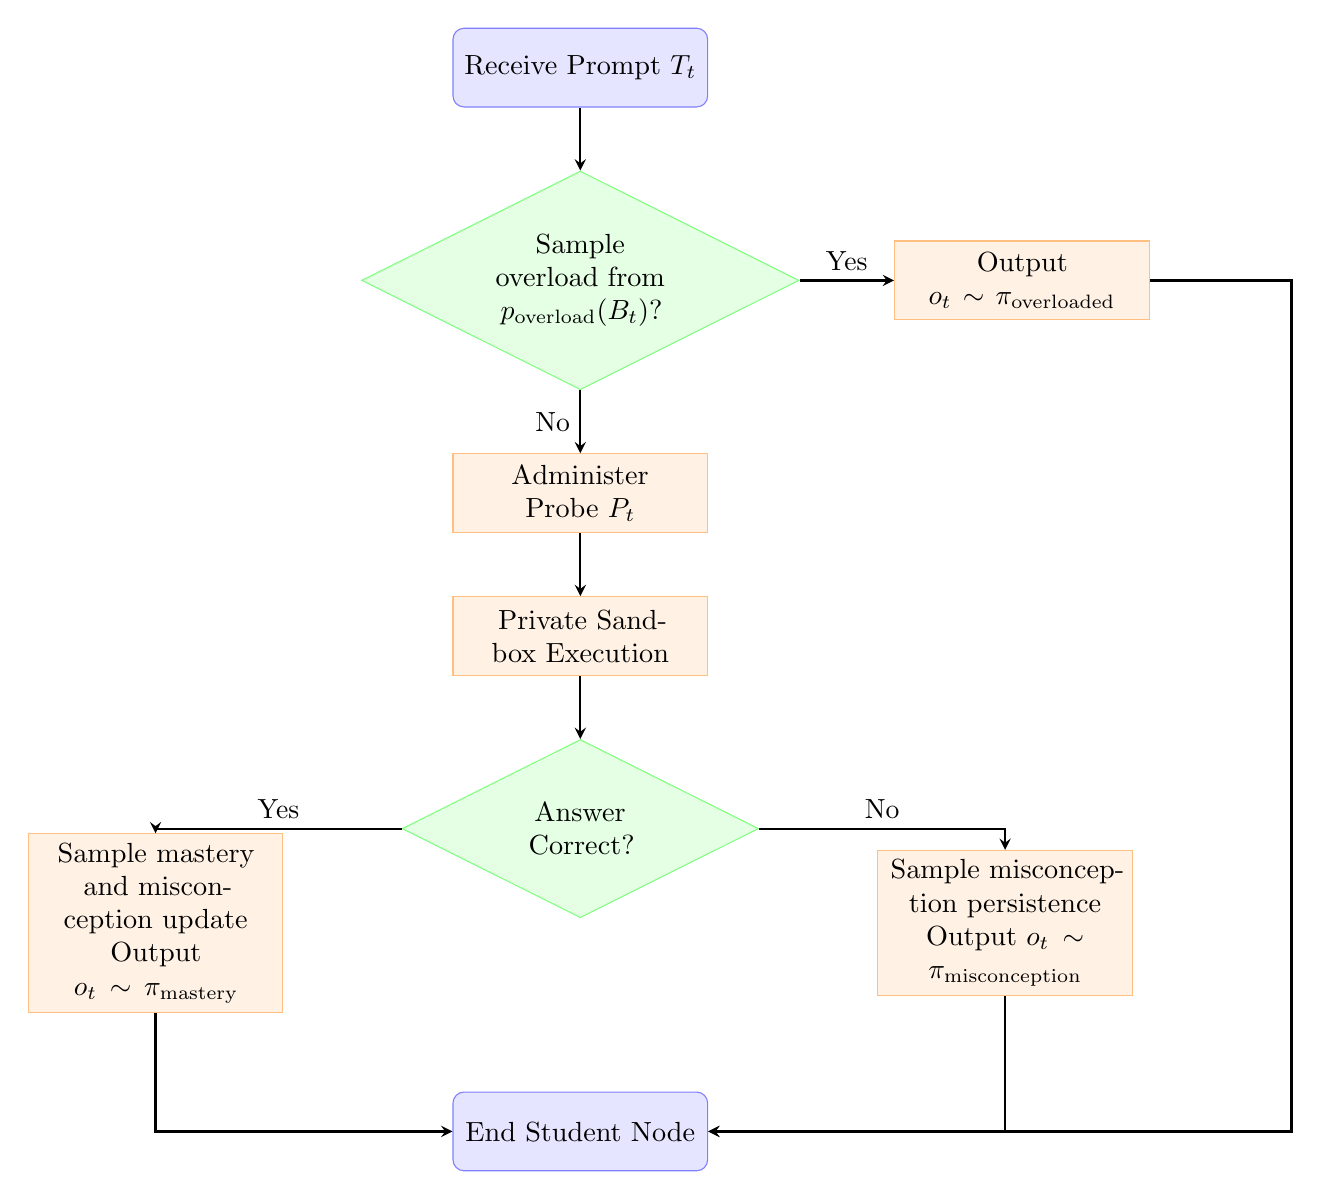
\begin{tikzpicture}[node distance=1.6cm, >=stealth]
    \node (start) [startstop] {Receive Prompt $T_t$};
    \node (check) [decision, below=0.8cm of start] {Sample overload from $p_{\text{overload}}(B_t)$?};
    \node (overloaded) [process, right=1.2cm of check] {Output $o_t \sim \pi_{\text{overloaded}}$};
    \node (probe) [process, below=0.8cm of check] {Administer Probe $P_t$};
    \node (scratch) [process, below=0.8cm of probe] {Private Sandbox Execution};
    \node (pass) [decision, below=0.8cm of scratch] {Answer Correct?};
    \node (mastery) [process, left=1.5cm of pass, yshift=-1.2cm] {Sample mastery and misconception update\\Output $o_t \sim \pi_{\text{mastery}}$};
    \node (misc) [process, right=1.5cm of pass, yshift=-1.2cm] {Sample misconception persistence\\Output $o_t \sim \pi_{\text{misconception}}$};
    \node (end) [startstop, below=2.2cm of pass] {End Student Node};
    
    \draw [arrow] (start) -- (check);
    \draw [arrow] (check) -- node[midway, above] {Yes} (overloaded);
    \draw [arrow] (check) -- node[midway, left] {No} (probe);
    \draw [arrow] (probe) -- (scratch);
    \draw [arrow] (scratch) -- (pass);
    \draw [arrow] (pass) -| (mastery) node[pos=0.25, above] {Yes};
    \draw [arrow] (pass) -| (misc) node[pos=0.25, above] {No};
    \draw [arrow] (mastery) |- (end);
    \draw [arrow] (misc) |- (end);
    \draw [arrow] (overloaded.east) -- ++(1.8,0) |- (end);
\end{tikzpicture}
}
\caption{Adversarial Probing and Sandbox Execution inside the Simulated Student Node.}
\label{fig:bottleneck}
\end{figure}

\chapter{Technical Achievements and Early Experimentation}
\label{ch:tech}

\section{LangGraph Orchestrator Flow}
The system is orchestrated via a centralised, versioned state buffer managed through a cyclic directed graph. To prevent write conflicts and preserve transaction integrity across asynchronous agent steps, state ownership is split explicitly: the simulator environment owns and mutates $s_t^{\text{true}}$ during synthetic experiments, while the Epistemic Tracker $A_e$ is the only component authorised to commit belief estimates $(\hat{\mathbf{K}}_t,\hat{\mathbf{M}}_t,\hat{B}_t,\hat{F}_t)$ to the tutor-facing buffer \cite{intellicode2025,elhaimeur2026itas}. The Socratic Tutor $A_t$ and Guardrail $A_g$ operate over read-only snapshots of tracker estimates and evidence. To investigate peer-agent social scaffolding dynamics (RQ2), the orchestrator stochastically instantiates a peer student agent $A_{\text{peer}}$ alongside the target student $A_s$. This peer agent introduces controlled conceptual or arithmetic errors into the dialogue, triggering productive cognitive conflict and observational learning---effects that recent social learning research demonstrates to enhance mastery acquisition \cite{kumar2026beyond}. As illustrated in Figure~\ref{fig:flowchart}, each cycle begins with the Epistemic Tracker ($A_e$) updating the learner belief state, followed by the Socratic Tutor ($A_t$) generating a pedagogical response, which is then routed through the Pedagogical Guardrail ($A_g$). The guardrail audits whether the response contains a direct answer or raw solution code; if so, it intercepts the output and dispatches it to a rewrite node that regenerates a Socratic question. Once a compliant response is produced, it is forwarded to the Simulated Student ($A_s$). The cycle terminates when the maximum turn count is reached or the student's mastery vector satisfies the completion criterion.
\begin{figure}[htbp]
\centering
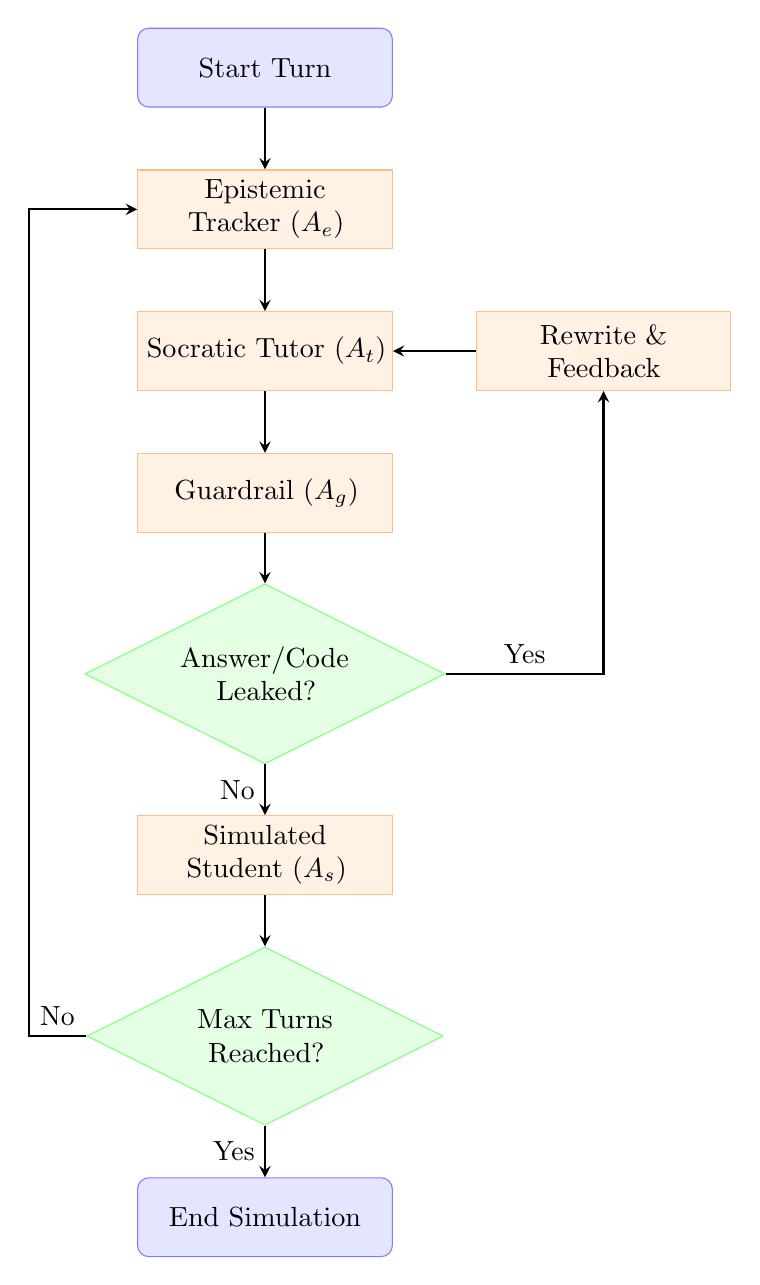
\begin{tikzpicture}[node distance=1.8cm]
    \node (start) [startstop] {Start Turn};
    \node (ae) [process, below of=start] {Epistemic Tracker ($A_e$)};
    \node (at) [process, below of=ae] {Socratic Tutor ($A_t$)};
    \node (ag) [process, below of=at] {Guardrail ($A_g$)};
    \node (dec) [decision, below of=ag, yshift=-0.5cm] {Answer/Code Leaked?};
    \node (rewrite) [process, right of=at, xshift=2.5cm] {Rewrite \& Feedback};
    \node (as) [process, below of=dec, yshift=-0.5cm] {Simulated Student ($A_s$)};
    \node (check) [decision, below of=as, yshift=-0.5cm] {Max Turns Reached?};
    \node (stop) [startstop, below of=check, yshift=-0.5cm] {End Simulation};
    
    \draw [arrow] (start) -- (ae);
    \draw [arrow] (ae) -- (at);
    \draw [arrow] (at) -- (ag);
    \draw [arrow] (ag) -- (dec);
    \draw [arrow] (dec) -- node[midway, left] {No} (as);
    \draw [arrow] (dec) -| (rewrite) node[pos=0.25, above] {Yes};
    \draw [arrow] (rewrite) -- (at);
    \draw [arrow] (as) -- (check);
    \draw [arrow] (check) -- node[midway, left] {Yes} (stop);
    \draw [arrow] (check) -- node[midway, above] {No} ++(-3,0) |- (ae);
\end{tikzpicture}
\caption{LangGraph Multi-Agent Cycle with Guardrail and State Loop.}
\label{fig:flowchart}
\end{figure}

\section{Structured State Definition}
The graph state and execution schema are implemented using Pydantic models, enforcing strict type validation at every LLM interface boundary, as detailed in Listing~\ref{lst:state}.

\begin{lstlisting}[language=Python, caption={LangGraph State Schema Definition with Cognitive Models.}, label={lst:state}]
from typing import List, Dict, Optional, TypedDict
from pydantic import BaseModel, Field, confloat

UnitFloat = confloat(ge=0.0, le=1.0)

class CognitiveState(BaseModel):
    bandwidth: UnitFloat = Field(default=1.0, description="B_t")
    overload_friction: UnitFloat = Field(default=0.0, description="F_t")
    underchallenge: UnitFloat = Field(default=0.0, description="F_t_minus")

class TrueStudentState(BaseModel):
    # Simulator-owned only; never exposed as policy input.
    mastery_vector: Dict[str, UnitFloat] = Field(default_factory=dict)
    misconceptions: Dict[str, bool] = Field(default_factory=dict)
    cognitive: CognitiveState = Field(default_factory=CognitiveState)

class TrackerEstimates(BaseModel):
    estimated_mastery: Dict[str, UnitFloat] = Field(default_factory=dict)
    misconception_marginals: Dict[str, UnitFloat] = Field(default_factory=dict)
    estimated_cognitive: CognitiveState = Field(default_factory=CognitiveState)
    effective_sample_size: float = 0.0
    posterior_uncertainty: Dict[str, float] = Field(default_factory=dict)

class LoadProxySignals(BaseModel):
    # Observable components used to construct Y_t^load.
    clarification_requested: bool = False
    confusion_marker: bool = False
    post_hint_probe_failed: bool = False
    high_edit_distance: bool = False
    latency_outlier: Optional[bool] = None
    expert_overload: Optional[bool] = None
    response_latency_ms: Optional[float] = None
    normalized_edit_distance: Optional[float] = None
    load_label: Optional[bool] = None

class ObservationEvidence(BaseModel):
    student_text: str = ""
    execution_passed: Optional[bool] = None
    probe_passed: Optional[bool] = None
    guardrail_leakage: bool = False
    prompt_load: Dict[str, float] = Field(default_factory=dict)
    load_proxy: LoadProxySignals = Field(default_factory=LoadProxySignals)

class TutorGuardrailOutput(BaseModel):
    is_valid: bool = Field(description="True if response avoids answer/code leakage")
    reason: str = Field(description="Pedagogical explanation for rejection")
    suggested_rewrite: str = Field(description="A Socratic version of the prompt")

class GraphState(TypedDict):
    conversation_history: List[Dict[str, str]]
    true_student_state: TrueStudentState
    tracker_estimates: TrackerEstimates
    latest_evidence: ObservationEvidence
    pedagogical_directives: List[str]
    turn_counter: int
    guardrail_warnings: int
    latest_tutor_response: str
\end{lstlisting}

\section{Algorithmic Formalisation}
This section operationalises the mathematical models introduced in Chapter~2, translating the POMDP formulation and cognitive state equations into a precise algorithmic specification. Algorithm~\ref{alg:langgraph_cycle} delineates the full execution cycle of the LangGraph orchestrator, detailing the information flow among the Epistemic Tracker ($A_e$), Socratic Tutor ($A_t$), Pedagogical Guardrail ($A_g$), and Simulated Student ($A_s$).

\begin{algorithm}[p]
\caption{LangGraph Multi-Agent Educational Simulation Cycle}
\label{alg:langgraph_cycle}
\footnotesize
\begin{algorithmic}[1]
\Require{Programming task $C$, maximum dialogue turns $T$, initial learner mastery vector $\mathbf{K}_0$, initial active misconceptions $\mathbf{M}_0$, cognitive parameters $(\lambda_c,\lambda_l,\lambda_f,\mu_r,\beta_+,\theta_{\text{overload}})$, maximum guardrail rewrites $N_{\text{rewrite}}$}
\Ensure{Dialogue history $H_T$, finalised true student profile $s^{\text{true}}_T$, compilation of learning metrics}
\State Initialise $H_0 \gets \emptyset$, cognitive bandwidth $B_0 \gets 1.0$, cognitive friction $F_0 \gets 0.0$, $W_0\gets0$, $n_{\text{fail}}\gets0$, turn $t \gets 1$
\State Initialise true student state: $\mathbf{K}_1^{\text{true}} \gets \mathbf{K}_0$, $\mathbf{M}_1^{\text{true}} \gets \mathbf{M}_0$, $s^{\text{true}}_1 \gets (\mathbf{K}_1^{\text{true}}, \mathbf{M}_1^{\text{true}}, B_0, F_0)$
\State Initialise tracker belief $b_1(s)$ representing the prior distribution
\While{$t \le T$ \textbf{and} $\mathbf{K}_{t}^{\text{true}} \neq \mathbf{1}$}
    \State \textit{// Step 1: Epistemic State Tracking ($A_e$)}
    \State Observe previous evidence bundle $e_{t-1}$ (if $t > 1$)
    \If{$t > 1$}
        \State Update belief state using SMC approximation to:
        \State $b_t(s') \gets \eta\int_{\mathcal{S}}\mathcal{T}(s'\mid\tilde{s}(s,u_{t-1}),u_{t-1},e_{t-1})$
        \Statex \hspace{\algorithmicindent}$\qquad\cdot\mathcal{Z}(e_{t-1}\mid\tilde{s}(s,u_{t-1}),u_{t-1})b_{t-1}(s)\,ds$
        \State Extract $\hat{\mathbf{K}}_t$, misconception marginals $\hat{\mathbf{p}}^M_t$, $\hat{\mathbf{M}}_t$, $\hat{B}_t$, and $\hat{F}_t$
    \Else
        \State Extract initial estimates from prior: $\hat{\mathbf{K}}_1$, $\hat{\mathbf{p}}^M_1$, $\hat{\mathbf{M}}_1$, $\hat{B}_1$, $\hat{F}_1$
    \EndIf
    
    \State \textit{// Step 2: Socratic Tutor Policy Planning ($A_t$)}
    \State Select directive and target concept using tracker-visible estimates:
    \State $(a_t,q_t) \gets \text{SelectPedagogicalDirective}(\hat{\mathbf{K}}_t,\hat{\mathbf{M}}_t,\hat{B}_t,\hat{F}_t,n_{\text{fail}},W_{t-1})$
    
    \State \textit{// Step 3: Pedagogical Guardrail Filtering ($A_g$)}
    \State Initialise rewrite counter $k \gets 0$, $\text{Passed} \gets \text{False}$
    \While{$k < N_{\text{rewrite}}$ \textbf{and} not $\text{Passed}$}
        \State Generate candidate tutor response: $T^{\text{cand}}_t \sim \pi_{\text{tutor}}(H_{t-1}, a_t, q_t)$
        \State Run Guardrail evaluation: $(is\_valid, reason, T^{\text{suggest}}) \gets \text{CheckGuardrails}(T^{\text{cand}}_t, C)$
        \If{$is\_valid$}
            \State $T_t \gets T^{\text{cand}}_t$
            \State $\text{Passed} \gets \text{True}$
        \Else
            \State $k \gets k + 1$
            \State Provide rejection reasons and $T^{\text{suggest}}$ as feedback to $A_t$
        \EndIf
    \EndWhile
    \If{not $\text{Passed}$}
        \State Fallback: $T_t \gets \text{GetTemplateSocraticQuery}(\hat{\mathbf{M}}_t)$
        \State Increment guardrail warning counter: $W_t \gets 1$
    \Else
        \State $W_t \gets 0$
    \EndIf
    
    \State \textit{// Step 4: Cognitive State Updates (using true student states)}
    \State $\ell_t \gets \text{ComputePromptLoadFeatures}(T_t)$
    \State $L_t \gets \text{ComputePromptLoad}(\ell_t)$, \quad
           $N_{\text{concepts},t}\gets\text{ExtractConceptCount}(T_t)$
    \State $Z_{\text{tutor},t}\gets\text{Difficulty}(T_t)$, \quad
           $Z_{\text{student},t}\gets K^{\text{true}}_{q_t,t}$
    \State $\Delta_t\gets Z_{\text{tutor},t}-Z_{\text{student},t}$
    \State $F_t \gets 1-\exp(-\beta_+\max(0,\Delta_t-\delta_{\text{zpd}}))$
    \State $D_t\gets\exp(-\lambda_cN_{\text{concepts},t}-\lambda_lL_t-\lambda_fF_t)$
    \State $B_t\gets\Pi_{[0,1]}(B_{t-1}D_t+\mu_r(1-B_{t-1})+\xi_t^B)$
    \State $u_t\gets(a_t,q_t,T_t,\ell_t,Z_{\text{tutor},t})$
    
    \State \textit{// Step 5: Simulated Student Execution ($A_s$)}
    \State Execute Student response selection with private adversarial probe (see Algorithm~\ref{alg:student_probing})
    \State Student generates response and updates true state:
    \State $e_t, \mathbf{K}_{t+1}^{\text{true}}, \mathbf{M}_{t+1}^{\text{true}} \gets \text{ExecuteStudentPolicy}(u_t,W_t,\mathbf{K}_t^{\text{true}},\mathbf{M}_t^{\text{true}},B_t,F_t)$
    \State $o_t \gets e_t.\text{student\_text}$
    \State Update repeated-failure counter $n_{\text{fail}}$ from $e_t.\text{probe\_passed}$, execution telemetry, and $e_t.\text{load\_proxy}$
    \State Append conversation: $H_t \gets H_{t-1} \cup \{(T_t, o_t)\}$
    \State Increment turn counter: $t \gets t + 1$
\EndWhile
\State \Return $H_{t-1}$, $(\mathbf{K}_{t}^{\text{true}}, \mathbf{M}_{t}^{\text{true}}, B_{t-1}, F_{t-1})$
\end{algorithmic}
\end{algorithm}

Algorithm~\ref{alg:student_probing} specifies the internal reasoning structure of the Simulated Student agent ($A_s$), formalising the adversarial information bottleneck that enforces consistency between the student's public dialogue output and its latent mastery state.

\begin{algorithm}[p]
\caption{Private Adversarial Scratchpad Probing \& Student Response Selection}
\label{alg:student_probing}
\small
\begin{algorithmic}[1]
\Require{Structured tutor control $u_t=(a_t,q_t,T_t,\ell_t,Z_{\text{tutor},t})$, guardrail flag $W_t$, true latent mastery vector $\mathbf{K}_t^{\text{true}}$, active misconceptions $\mathbf{M}_t^{\text{true}}$, student cognitive state $(B_t,F_t)$, private diagnostic probe generator $\mathcal{P}$, response policies $\{\pi_{\text{mastery}}, \pi_{\text{misconception}}, \pi_{\text{overloaded}}\}$}
\Ensure{Evidence bundle $e_t$, updated latent mastery vector $\mathbf{K}_{t+1}^{\text{true}}$, updated misconception vector $\mathbf{M}_{t+1}^{\text{true}}$}
\State \textit{// Step 1: Administer Private Diagnostic Probe}
\State Generate a targeted private coding query and misconception target: $(P_t,c_t) \sim \mathcal{P}(\mathbf{M}_t^{\text{true}},q_t)$
\State \textit{// Step 2: Private Execution in Scratchpad (Decoupled from Public Dialogue)}
\State Instantiate a private scratchpad telemetry record: $S_t^{\text{diag}} \gets \emptyset$
\State Generate a private solution attempt and final answer candidate $A^{\text{cand}}_t$:
\State $S_t^{\text{diag}}, A^{\text{cand}}_t \gets \text{GeneratePrivateAttempt}(P_t, \mathbf{K}_t^{\text{true}}, \mathbf{M}_t^{\text{true}})$
\State Execute code or evaluate answer: $y_t \gets \text{ExecutePrivateAnswer}(A^{\text{cand}}_t)$
\State Collect execution telemetry: $x_t^{\text{exec}}\gets\text{CollectExecutionTelemetry}(A^{\text{cand}}_t,y_t)$
\State Retrieve ground-truth answer for probe: $y^*_t$
\State \textit{// Step 3: Conditional Policy Enforcement (Information Bottleneck)}
\State Draw cognitive overload state indicator $S_{\text{overload}} \sim \text{Bernoulli}(p_{\text{overload}}(B_t))$, where $p_{\text{overload}}(B_t)$ decreases as $B_t$ increases
\If{$S_{\text{overload}} == 1$}
    \State \textit{// Cognitive overload overrides standard reasoning}
    \State Generate public response: $o_t \sim \pi_{\text{overloaded}}(T_t, B_t, F_t)$
\Else
    \If{$y_t == y^*_t$}
        \State \textit{// Probe passed: demonstrated performance evidence}
        \State Generate public response: $o_t \sim \pi_{\text{mastery}}(T_t, S_t^{\text{diag}})$
    \Else
        \State \textit{// Probe Failed: Misconception active}
        \State Generate public response: $o_t \sim \pi_{\text{misconception}}(T_t, S_t^{\text{diag}}, \mathbf{M}_t^{\text{true}})$
    \EndIf
\EndIf
\State $\psi_t \gets
    \text{ComputeLoadProxySignals}(o_t,y_t==y_t^*,W_t,\ell_t,S_{\text{overload}})$
\State Package evidence bundle:
       $e_t\gets(o_t,x_t^{\text{exec}},y_t==y_t^*,W_t,\psi_t)$
\State \textit{// Step 4: True Latent State Transitions (Probabilistic Simulator Dynamics)}
\State $\Delta_t \gets Z_{\text{tutor},t}-K^{\text{true}}_{q_t,t}$
\State $\mathbf{K}_{t+1}^{\text{true}} \gets
    \text{UpdateMasteryVector}(\mathbf{K}_t^{\text{true}},q_t,B_t,F_t,\Delta_t)$
\State $\mathbf{M}_{t+1}^{\text{true}} \gets
    \text{SampleMisconceptionTransition}(\mathbf{M}_t^{\text{true}},c_t,y_t==y_t^*,B_t,F_t)$
\State \Return $e_t$, $\mathbf{K}_{t+1}^{\text{true}}$, $\mathbf{M}_{t+1}^{\text{true}}$
\end{algorithmic}
\end{algorithm}

\subsection{Mathematical Convergence and Resampling Proof}
This section establishes a finite-horizon consistency justification for the Sequential Monte Carlo (SMC) particle filter under Laplace-smoothed likelihoods and systematic resampling. The analysis shows that smoothing prevents zero-likelihood degeneracy and that, for any fixed dialogue horizon, the particle approximation converges as $M$ increases. It does not claim that particle filtering validates the simulator's psychological assumptions or prevents all long-horizon filter degeneracy.

Let $\mathcal{S}$ denote the latent student state space, and let $s_{1:t} = (s_1, \dots, s_t) \in \mathcal{S}^t$ represent the historical trajectory of true student states up to turn $t$. Let $o_{1:t} = (o_1, \dots, o_t) \in \mathcal{O}^t$ denote the observed sequence of natural language dialogue and programming actions. The true posterior distribution of the student state at turn $t$ is denoted by $p(s_t \mid o_{1:t})$. The SMC filter approximates this posterior with an empirical distribution $p^M(s_t \mid o_{1:t})$ represented by a set of $M$ weighted particles $\{ (s_t^{[i]}, W_t^{[i]}) \}_{i=1}^M$, where:
\begin{equation}
    p^M(s_t \mid o_{1:t}) = \sum_{i=1}^M W_t^{[i]} \delta_{s_t^{[i]}}(s_t)
\end{equation}
where $\delta_{s_t^{[i]}}$ is the Dirac delta measure centred at $s_t^{[i]}$, and $W_t^{[i]} \ge 0$ are the normalised importance weights satisfying $\sum_{i=1}^M W_t^{[i]} = 1$.

\subsubsection{Weight Variance and Laplace Smoothing Bounding}
In standard particle filtering, the importance weight update at turn $t$ is determined by the observation likelihood:
\begin{equation}
    w_t^{[i]} = W_{t-1}^{[i]} \cdot \mathcal{Z}(o_t \mid s_t^{[i]}, a_t)
\end{equation}
When the student output $o_t$ is anomalous or indicative of a misconception highly improbable under the transition model for a given particle, the raw likelihood $\mathcal{Z}(o_t \mid s_t^{[i]}, a_t)$ approaches zero. Under sequential multiplicative updates, this causes all weight to concentrate on a single particle, yielding $N_{\text{eff}} \to 1$---the particle collapse failure mode.

To prevent this degeneration, the Epistemic Tracker applies Laplace smoothing to the observation likelihood. Letting $\mathcal{Z}_{\text{raw}}(o_t \mid s_t^{[i]}, a_t)$ denote the raw likelihood from the semantic classifier, the smoothed likelihood is defined as:
\begin{equation}
    \mathcal{Z}_{\text{smooth}}(o_t \mid s_t^{[i]}, a_t) = (1 - \alpha_{\text{smooth}}) \mathcal{Z}_{\text{raw}}(o_t \mid s_t^{[i]}, a_t) + \alpha_{\text{smooth}} \epsilon_{\text{smooth}}
\end{equation}
where $\alpha_{\text{smooth}} \in (0, 1)$ represents the smoothing coefficient and $\epsilon_{\text{smooth}} > 0$ denotes a uniform prior over the observation space. 

\begin{theorem}[Uniformly Bounded Weights]
Under Laplace smoothing, the unnormalised particle weights are bounded above and below by positive constants independent of the observation history:
\begin{equation}
    0 < c_{\text{min}} \le w_t^{[i]} \le c_{\text{max}} < \infty
\end{equation}
for all $i \in \{1, \dots, M\}$ and $t \ge 1$.
\end{theorem}

\begin{proof}
Since $\mathcal{Z}_{\text{raw}}(o_t \mid s_t^{[i]}, a_t) \le 1$ and $\epsilon_{\text{smooth}} \le 1$, we have:
\begin{equation}
    \mathcal{Z}_{\text{smooth}}(o_t \mid s_t^{[i]}, a_t) \le (1 - \alpha_{\text{smooth}}) \cdot 1 + \alpha_{\text{smooth}} \epsilon_{\text{smooth}} \le 1
\end{equation}
Hence, the maximum likelihood is bounded. Conversely, since $\mathcal{Z}_{\text{raw}}(o_t \mid s_t^{[i]}, a_t) \ge 0$, the smoothed likelihood is bounded strictly from below:
\begin{equation}
    \mathcal{Z}_{\text{smooth}}(o_t \mid s_t^{[i]}, a_t) \ge \alpha_{\text{smooth}} \epsilon_{\text{smooth}} > 0
\end{equation}
Assuming that the particles at step $t-1$ were resampled and normalised such that $W_{t-1}^{[i]} \in [\frac{1}{M c_{\text{scale}}}, \frac{c_{\text{scale}}}{M}]$, the unnormalised weights $w_t^{[i]} = W_{t-1}^{[i]} \mathcal{Z}_{\text{smooth}}(o_t \mid s_t^{[i]}, a_t)$ satisfy:
\begin{equation}
    w_t^{[i]} \ge \frac{\alpha_{\text{smooth}} \epsilon_{\text{smooth}}}{M c_{\text{scale}}} > 0 \quad \text{and} \quad w_t^{[i]} \le \frac{c_{\text{scale}}}{M}
\end{equation}
Setting $c_{\text{min}} = \frac{\alpha_{\text{smooth}} \epsilon_{\text{smooth}}}{M c_{\text{scale}}}$ and $c_{\text{max}} = \frac{c_{\text{scale}}}{M}$ yields the bounds.
\end{proof}

This uniform bound is then used to establish a positive lower bound on the effective sample size $N_{\text{eff}}$, precluding instantaneous collapse.
\begin{corollary}[Non-vanishing Effective Sample Size]
The effective sample size $N_{\text{eff}}$ is bounded from below by a positive constant:
\begin{equation}
    N_{\text{eff}} \ge M \left( \frac{\alpha_{\text{smooth}} \epsilon_{\text{smooth}}}{c_{\text{scale}}^2} \right)^2 > 0
\end{equation}
preventing instantaneous particle collapse.
\end{corollary}

\begin{proof}
Recall the definition of the normalised weights:
\begin{equation}
    W_t^{[i]} = \frac{w_t^{[i]}}{\sum_{j=1}^M w_t^{[j]}}
\end{equation}
Applying the bounds from Theorem 1:
\begin{equation}
    \sum_{j=1}^M w_t^{[j]} \le M c_{\text{max}}
\end{equation}
Thus, the normalised weights are bounded from below:
\begin{equation}
    W_t^{[i]} \ge \frac{c_{\text{min}}}{M c_{\text{max}}}
\end{equation}
Substituting this into the expression for $N_{\text{eff}}$:
Because $W_t^{[i]} \le \frac{c_{\text{max}}}{M c_{\text{min}}}$, it follows that:
\begin{equation}
    \sum_{i=1}^M (W_t^{[i]})^2 \le M \left( \frac{c_{\text{max}}}{M c_{\text{min}}} \right)^2 = \frac{c_{\text{max}}^2}{M c_{\text{min}}^2}
\end{equation}
Taking the reciprocal yields:
\begin{equation}
    N_{\text{eff}} = \frac{1}{\sum_{i=1}^M (W_t^{[i]})^2} \ge M \left( \frac{c_{\text{min}}}{c_{\text{max}}} \right)^2
\end{equation}
Substituting $c_{\text{min}}$ and $c_{\text{max}}$ gives:
\begin{equation}
    N_{\text{eff}} \ge M \left( \frac{\alpha_{\text{smooth}} \epsilon_{\text{smooth}}}{c_{\text{scale}}^2} \right)^2
\end{equation}
which is independent of the observation $o_t$ and strictly positive.
\end{proof}

\subsubsection{Resampling Variance and Systematic Resampling Recurrence}
When $N_{\text{eff}} < \theta_{\text{resample}}$, we perform systematic resampling. Let $C_k = \sum_{j=1}^k W_t^{[j]}$ be the cumulative sum of normalized weights, with $C_0 = 0$. Systematic resampling draws a single random variable $U \sim \mathcal{U}([0, 1/M))$ and constructs the grid points:
\begin{equation}
    u_i = U + \frac{i-1}{M}, \quad \text{for } i = 1, \dots, M
\end{equation}
The resampled particle index $j^*(i)$ for the $i$-th new particle is selected according to:
\begin{equation}
    j^*(i) = \{ j : u_i \in [C_{j-1}, C_j) \}
\end{equation}

\begin{theorem}[Variance Reduction of Systematic Resampling]
Let $N_j = \sum_{i=1}^M \mathbb{I}(j^*(i) == j)$ be the number of copies of particle $j$ selected during resampling. Under systematic resampling, the variance of $N_j$ is strictly bounded and satisfies:
\begin{equation}
    \text{Var}(N_j)=\delta_j(1-\delta_j)\le\frac{1}{4},
\end{equation}
where $\delta_j$ is the fractional part of $MW_t^{[j]}$. This is bounded independently of $M$ and is smaller than the multinomial count variance $\text{Var}_{\text{multi}}(N_j)=MW_t^{[j]}(1-W_t^{[j]})$ for high-count particles.
\end{theorem}

\begin{proof}
Under systematic resampling, the number of selection points $u_i$ falling within the interval $[C_{j-1}, C_j)$ depends on the interval length $W_t^{[j]} = C_j - C_{j-1}$. Since the distance between consecutive grid points $u_i$ is exactly $1/M$, the number of grid points that can fall into an interval of length $W_t^{[j]}$ is highly constrained. Specifically, it must satisfy:
\begin{equation}
    \lfloor M W_t^{[j]} \rfloor \le N_j \le \lceil M W_t^{[j]} \rceil
\end{equation}
Let $M W_t^{[j]} = k_j + \delta_j$, where $k_j = \lfloor M W_t^{[j]} \rfloor$ is an integer and $\delta_j \in [0, 1)$ is the fractional part. The random variable $N_j$ can only take two values: $k_j$ with probability $1 - \delta_j$, and $k_j + 1$ with probability $\delta_j$. The expected value is:
\begin{equation}
    \mathbb{E}[N_j] = k_j (1 - \delta_j) + (k_j + 1) \delta_j = k_j + \delta_j = M W_t^{[j]}
\end{equation}
The variance is given by:
\begin{equation}
    \text{Var}(N_j) = \mathbb{E}[N_j^2] - (\mathbb{E}[N_j])^2 = \delta_j (1 - \delta_j)
\end{equation}
Since $\delta_j < 1$, we have:
\begin{equation}
    \text{Var}(N_j) = \delta_j (1 - \delta_j) \le \frac{1}{4}
\end{equation}
which is a constant, independent of the number of particles $M$. In contrast, for multinomial resampling, the number of copies $N_j$ follows a binomial distribution $\text{Binomial}(M, W_t^{[j]})$, which has variance:
\begin{equation}
    \text{Var}_{\text{multi}}(N_j) = M W_t^{[j]} (1 - W_t^{[j]})
\end{equation}
For large $M$, $\text{Var}_{\text{multi}}(N_j)$ grows linearly with $M$ (relative to the target count $M W_t^{[j]}$), which introduces significant high-frequency noise into the particle set and degrades the accuracy of subsequent state transitions. Systematic resampling eliminates this $M$-dependent noise.
\end{proof}

\subsubsection{Overall Particle Filter Convergence Rate}
Combining the bounds established above, we use the standard finite-horizon particle-filter consistency result: for each fixed turn $t$, the particle approximation $p^M(s_t \mid o_{1:t})$ converges to the posterior $p(s_t \mid o_{1:t})$ with mean-squared error $O(1/M)$ as $M \to \infty$.

Let $B(\mathcal{S})$ denote the space of bounded, measurable, real-valued test functions on $\mathcal{S}$. For any $\phi \in B(\mathcal{S})$, define:
\begin{equation}
    (p_t, \phi) = \int_{\mathcal{S}} \phi(s_t) p(s_t \mid o_{1:t}) ds_t \quad \text{and} \quad (p_t^M, \phi) = \sum_{i=1}^M W_t^{[i]} \phi(s_t^{[i]})
\end{equation}

\begin{theorem}[Finite-Horizon $L_2$ Consistency of the Epistemic Tracker]
Assume $\mathcal{S}$ is compact, the transition kernel $\mathcal{T}$ satisfies the Feller property, and the smoothed observation likelihood is bounded and strictly positive, $0<\underline{z}\le \mathcal{Z}_{\text{smooth}}\le\bar{z}<\infty$. For any fixed horizon $T<\infty$, any $t\le T$, and any $\phi\in B(\mathcal{S})$, there exists a constant $C_t<\infty$ independent of $M$ such that:
\begin{equation}
    \mathbb{E}\left[ \left| (p_t^M, \phi) - (p_t, \phi) \right|^2 \right] \le \frac{C_t}{M} \parallel \phi \parallel^2
\end{equation}
where $\parallel \phi \parallel = \sup_{s \in \mathcal{S}} |\phi(s)|$. The constant $C_t$ may grow with $t$ and with $\underline{z}^{-1}$.
\end{theorem}

\begin{proof}
The proof proceeds by induction on $t$. For $t = 1$, particles are sampled i.i.d.\ from the prior $p(s_1)$, and the bound follows from the classical Law of Large Numbers, with $C_1 = 1$.

Assume the induction hypothesis holds for $t-1$, i.e., $\mathbb{E}\left[ \left| (p_{t-1}^M, \phi) - (p_{t-1}, \phi) \right|^2 \right] \le \frac{C_{t-1}}{M} \parallel \phi \parallel^2$.
At turn $t$, the update consists of a prediction step followed by a correction step. Let $p_{t-1 \to t}$ be the predicted distribution:
\begin{equation}
    p_{t-1 \to t}(s_t) = \int_{\mathcal{S}} \mathcal{T}(s_t \mid s_{t-1}) p(s_{t-1} \mid o_{1:t-1}) ds_{t-1}
\end{equation}
and let $p_{t-1 \to t}^M$ be its particle approximation prior to observation:
\begin{equation}
    p_{t-1 \to t}^M(s_t) = \frac{1}{M} \sum_{i=1}^M \delta_{s_t^{[i]}}(s_t), \quad \text{where } s_t^{[i]} \sim \mathcal{T}(\cdot \mid s_{t-1}^{[i]})
\end{equation}
The correction step updates the distribution using the smoothed likelihood $\mathcal{Z}_{\text{smooth}}$. By the properties of importance sampling:
\begin{equation}
    (p_t, \phi) = \frac{(p_{t-1 \to t}, \phi \cdot \mathcal{Z}_{\text{smooth}})}{(p_{t-1 \to t}, \mathcal{Z}_{\text{smooth}})} \quad \text{and} \quad (p_t^M, \phi) = \frac{(p_{t-1 \to t}^M, \phi \cdot \mathcal{Z}_{\text{smooth}})}{(p_{t-1 \to t}^M, \mathcal{Z}_{\text{smooth}})}
\end{equation}
Let $f_1 = \phi \cdot \mathcal{Z}_{\text{smooth}}$ and $f_2 = \mathcal{Z}_{\text{smooth}}$. We decompose the estimation error:
\begin{equation}
    \begin{split}
        (p_t^M, \phi) - (p_t, \phi) &= \frac{(p_{t-1 \to t}^M, f_1)}{(p_{t-1 \to t}^M, f_2)} - \frac{(p_{t-1 \to t}, f_1)}{(p_{t-1 \to t}, f_2)} \\
        &= \frac{(p_{t-1 \to t}^M, f_1)(p_{t-1 \to t}, f_2) - (p_{t-1 \to t}^M, f_2)(p_{t-1 \to t}, f_1)}{(p_{t-1 \to t}^M, f_2)(p_{t-1 \to t}, f_2)}
    \end{split}
\end{equation}
By Theorem 1, $(p_{t-1 \to t}, f_2) \ge \alpha_{\text{smooth}} \epsilon_{\text{smooth}}$ and $(p_{t-1 \to t}^M, f_2) \ge \alpha_{\text{smooth}} \epsilon_{\text{smooth}}$. Thus, the denominator is strictly bounded away from zero. Setting $D = (p_{t-1 \to t}, f_2)(p_{t-1 \to t}^M, f_2) \ge (\alpha_{\text{smooth}} \epsilon_{\text{smooth}})^2$, we have:
\begin{equation}
    \left| (p_t^M, \phi) - (p_t, \phi) \right| \le \frac{1}{(\alpha_{\text{smooth}} \epsilon_{\text{smooth}})^2} \left| (p_{t-1 \to t}^M, f_1)(p_{t-1 \to t}, f_2) - (p_{t-1 \to t}^M, f_2)(p_{t-1 \to t}, f_1) \right|
\end{equation}
Adding and subtracting $(p_{t-1 \to t}, f_1)(p_{t-1 \to t}, f_2)$ inside the absolute value yields:
\begin{equation}
\begin{split}
    \left| (p_t^M, \phi) - (p_t, \phi) \right| \le \frac{1}{(\alpha_{\text{smooth}} \epsilon_{\text{smooth}})^2} & \left[ \left| (p_{t-1 \to t}^M, f_1) - (p_{t-1 \to t}, f_1) \right| \cdot (p_{t-1 \to t}, f_2) \right. \\
    & \left. + \left| (p_{t-1 \to t}^M, f_2) - (p_{t-1 \to t}, f_2) \right| \cdot (p_{t-1 \to t}, f_1) \right]
\end{split}
\end{equation}
Applying the inequality $(a+b)^2 \le 2a^2 + 2b^2$ and taking expectations:
\begin{equation}
\begin{split}
    \mathbb{E}\left[ \left| (p_t^M, \phi) - (p_t, \phi) \right|^2 \right] \le \frac{2}{(\alpha_{\text{smooth}} \epsilon_{\text{smooth}})^4} & \left[ \mathbb{E}\left[ \left| (p_{t-1 \to t}^M, f_1) - (p_{t-1 \to t}, f_1) \right|^2 \right] \cdot \parallel f_2 \parallel^2 \right. \\
    & \left. + \mathbb{E}\left[ \left| (p_{t-1 \to t}^M, f_2) - (p_{t-1 \to t}, f_2) \right|^2 \right] \cdot \parallel f_1 \parallel^2 \right]
\end{split}
\end{equation}
Since $\parallel f_2 \parallel = \parallel \mathcal{Z}_{\text{smooth}} \parallel \le 1$ and $\parallel f_1 \parallel = \parallel \phi \cdot \mathcal{Z}_{\text{smooth}} \parallel \le \parallel \phi \parallel$, we obtain:
\begin{equation}
    \begin{split}
        \mathbb{E}\left[ \left| (p_t^M, \phi) - (p_t, \phi) \right|^2 \right] &\le \frac{2 \parallel \phi \parallel^2}{(\alpha_{\text{smooth}} \epsilon_{\text{smooth}})^4} \left[ \mathbb{E}\left[ \left| (p_{t-1 \to t}^M, \bar{f}_1) - (p_{t-1 \to t}, \bar{f}_1) \right|^2 \right] \right. \\
        &\quad \left. + \mathbb{E}\left[ \left| (p_{t-1 \to t}^M, \bar{f}_2) - (p_{t-1 \to t}, \bar{f}_2) \right|^2 \right] \right]
    \end{split}
\end{equation}
where $\bar{f}_1 = f_1 / \parallel \phi \parallel$ has sup-norm at most 1. By the induction hypothesis and the Feller property of $\mathcal{T}$, both expectation terms on the right-hand side are bounded by $C'_{t-1}/M$ for a constant $C'_{t-1}$ depending only on $C_{t-1}$ and the transition dynamics. Consequently:
\begin{equation}
    \mathbb{E}\left[ \left| (p_t^M, \phi) - (p_t, \phi) \right|^2 \right] \le \frac{4 C'_{t-1}}{M (\alpha_{\text{smooth}} \epsilon_{\text{smooth}})^4} \parallel \phi \parallel^2
\end{equation}
Defining $C_t = \frac{4 C'_{t-1}}{(\alpha_{\text{smooth}} \epsilon_{\text{smooth}})^4}$ completes the inductive step.
\end{proof}
This theorem confirms that the SMC particle filter is a consistent finite-horizon estimator of hidden simulator states. The guarantee is conditional on the simulator transition and observation models; it does not establish that the latent variables are valid measurements of human cognition. Laplace smoothing keeps the normalising denominator positive, but small smoothing floors can still produce large constants, so empirical calibration and ablation remain necessary.

\section{Secure Execution Sandbox Architecture}
The system exposes a Python code execution sandbox via a Model Context Protocol (MCP) server, enabling real-time evaluation of student-submitted scripts. To preclude arbitrary code execution, resource exhaustion, and host environment compromise, the execution layer enforces a multi-layered containment strategy:
\begin{enumerate}
    \item \textbf{AST Whitelisting:} Prior to execution, all Python scripts are parsed into an Abstract Syntax Tree (AST) using the native \texttt{ast} module. The code is statically scanned and verified against a strict whitelist of permitted AST nodes (including control flow, assignments, and arithmetic operators). Any script containing import nodes (\texttt{Import}, \texttt{ImportFrom}), private attribute lookups (dunder attributes starting with \texttt{\_\_}), or restricted built-in primitives (\texttt{eval}, \texttt{exec}, \texttt{open}, \texttt{compile}) is immediately rejected with a security validation warning.
    \item \textbf{Process Isolation:} Execution is decoupled from the core LangGraph server. Code is executed inside an isolated sub-process spawned via the \texttt{multiprocessing} module. Communication with the parent server is restricted to a read-only serialisation queue, blocking socket reuse and memory corruption paths.
    \item \textbf{UNIX Resource Gating:} Within the spawned child process, kernel-level resource limits are enforced via the UNIX \texttt{resource} module:
    \begin{itemize}
        \item \textbf{CPU Time Limit (\texttt{RLIMIT\_CPU}):} Capped at $1.0$ second to prevent infinite loops.
        \item \textbf{Memory Space Limit (\texttt{RLIMIT\_AS}):} Capped at $50$ megabytes of virtual memory to mitigate memory exhaustion.
        \item \textbf{Process Limits (\texttt{RLIMIT\_NPROC}):} Capped at $0$ to block sub-process spawning and fork-bomb exploits.
    \end{itemize}
    \item \textbf{Timeout Watchdog:} A hard $1.0$-second timeout watchdog terminates the child process if it remains active beyond the limit, returning a compilation error rather than blocking the main execution threads.
\end{enumerate}
Together, these four layers constitute a zero-trust containment boundary on the host machine, and serve as a self-contained fallback when cloud-hosted microVM runtimes (such as E2B or Modal) are unavailable.

\subsection{AST Whitelist and Subprocess Containment Implementation}
This section details the static verification and process containment logic used when executing student code or simulated agent scripts on the local host. Listing~\ref{lst:sandbox_impl} presents the MCP server implementation, covering the AST whitelist traversal and the UNIX resource limit configuration.

\begin{lstlisting}[language=Python, caption={Python Code Sandbox AST Whitelisting and Subprocess Container.}, label={lst:sandbox_impl}]
import ast
import multiprocessing
import io
import contextlib
from typing import Tuple

def is_safe_ast(code: str) -> Tuple[bool, str]:
    """
    Parse code using Python's native AST parser and check against a whitelist 
    of nodes and a blacklist of unsafe modules and attributes.
    """
    try:
        tree = ast.parse(code)
    except Exception as e:
        return False, f"Syntax Error: {str(e)}"
        
    allowed_nodes = {
        ast.Module, ast.Assign, ast.Name, ast.Constant, ast.Expr, ast.Call, 
        ast.Attribute, ast.List, ast.Subscript, ast.BinOp, ast.UnaryOp, 
        ast.Compare, ast.Pass, ast.Break, ast.Continue, ast.If, ast.For, 
        ast.While, ast.FunctionDef, ast.arguments, ast.arg, ast.Return, 
        ast.Load, ast.Store, ast.Del, ast.Add, ast.Sub, ast.Mult, ast.Div,
        ast.Mod, ast.Pow, ast.LShift, ast.RShift, ast.BitOr, ast.BitXor, 
        ast.BitAnd, ast.FloorDiv, ast.USub, ast.UAdd, ast.Not, ast.Invert,
        ast.Eq, ast.NotEq, ast.Lt, ast.LtE, ast.Gt, ast.GtE, ast.Is, ast.IsNot,
        ast.In, ast.NotIn, ast.And, ast.Or, ast.BoolOp
    }
    
    # Backward compatibility for deprecated AST classes in older Python versions
    for name in ['Num', 'Str', 'Bytes', 'NameConstant', 'Index', 'ExtSlice']:
        if hasattr(ast, name):
            allowed_nodes.add(getattr(ast, name))
            
    blocked_builtins = {
        'eval', 'exec', 'open', 'compile', 'importlib', '__import__', 
        'globals', 'locals', 'getattr', 'setattr', 'delattr'
    }
    
    for node in ast.walk(tree):
        if type(node) not in allowed_nodes:
            return False, f"Disallowed syntax node type: {type(node).__name__}"
            
        # Enforce restricted built-in calls
        if isinstance(node, ast.Call):
            if isinstance(node.func, ast.Name) and node.func.id in blocked_builtins:
                return False, f"Call to blocked builtin function: {node.func.id}"
                
        # Block double-underscore attribute access to prevent sandbox escapes (e.g. __class__)
        if isinstance(node, ast.Attribute):
            if node.attr.startswith('__'):
                return False, f"Access to private attribute/dunder method: {node.attr}"
                
        # Block double-underscore identifiers
        if isinstance(node, ast.Name):
            if node.id.startswith('__'):
                return False, f"Access to restricted identifier: {node.id}"
                
    return True, ""


def child_process_executor(code: str, queue: multiprocessing.Queue) -> None:
    """
    Child process execution target. Redirects stdout/stderr and sets resource limits.
    """
    # Resource constraints (Unix/MacOS only)
    try:
        import resource
        # Limit CPU time to 1 second
        resource.setrlimit(resource.RLIMIT_CPU, (1, 1))
        # Limit memory address space to 50MB
        resource.setrlimit(resource.RLIMIT_AS, (50 * 1024 * 1024, 50 * 1024 * 1024))
        # Prevent fork bomb attacks by banning sub-processes
        resource.setrlimit(resource.RLIMIT_NPROC, (0, 0))
    except Exception:
        pass

    stdout_buf = io.StringIO()
    stderr_buf = io.StringIO()
    exit_code = 0
    
    # Establish a strictly sandboxed global namespace
    safe_builtins = {
        k: v for k, v in __builtins__.__dict__.items()
        if k not in {'open', 'eval', 'exec', 'compile', 'importlib', '__import__', 'globals', 'locals', 'getattr', 'setattr', 'delattr'}
    } if hasattr(__builtins__, '__dict__') else {}
    
    safe_globals = {"__builtins__": safe_builtins}
    local_scope = {}
    
    try:
        with contextlib.redirect_stdout(stdout_buf), contextlib.redirect_stderr(stderr_buf):
            exec(code, safe_globals, local_scope)
    except Exception as e:
        stderr_buf.write(str(e))
        exit_code = 1
        
    queue.put({
        "stdout": stdout_buf.getvalue(),
        "stderr": stderr_buf.getvalue(),
        "exit_code": exit_code
    })
\end{lstlisting}

\section{Early Experimental Logs and State Traces}

The following hand-worked traces illustrate the intended qualitative behaviour of the Cognitive Bandwidth and Friction equations ($B_t$, $F_t$) together with the Adversarial Scratchpad Probing protocol. They are sanity checks, not empirical validation; empirical support is provided only by the ablation and held-out evaluation protocol in Chapter~\ref{ch:plan}. For readability, these traces use a simplified deterministic load term based on raw prompt length rather than the full normalised \texttt{ComputePromptLoad} feature vector.

\subsection{Turn 1: Baseline State}
The student agent $A_s$ is initialised with a misconception conflating reference assignment with shallow copying.
\begin{itemize}
    \item \textbf{Tutor input ($T_1$):} ``Let's look at how Python handles variable assignment. If we set $x = [1,2,3]$ and $y = x$, what happens when we modify $y$?'' (Raw length feature $L^{\text{raw}}_1 = 120$ characters, $N_{\text{concepts},1} = 1$).
    \item \textbf{Cognitive Equations:}
    \begin{align*}
        B_1 &= 1.0 \cdot \exp\left(-0.1(1) - 0.001(120)\right) + 0.1(0) = 0.80 \\
        F_1 &= 1 - \exp\left(-0.5 \cdot \max(0, 0.4 - 0.3)\right) = 0.05
    \end{align*}
    \item \textbf{Adversarial Scratchpad Probe ($P_1$):} ``Evaluate: $x = [5]; y = x; y.\text{append}(2); \text{print}(x)$''.
    \item \textbf{Scratchpad Result:} $A_s$ private solver outputs $[5]$. (Failed: shows target misconception).
    \item \textbf{Internal Mastery:} $K^{\text{true}}_{\text{ref}, 1} = 0.0$ (Unmastered).
    \item \textbf{Public Response ($A_{s,1}$):} ``Only $y$ changes because $y$ is a new list. So $x$ remains $[5]$.''
\end{itemize}

\subsection{Turn 2: Cognitive Overload Trigger}
The Tutor node violates the Socratic constraint by generating an overloaded response that simultaneously introduces Python namespaces, memory layout, and garbage collection semantics.
\begin{itemize}
    \item \textbf{Tutor input ($T_2$):} ``Actually, variables in Python are just labels bound to objects. When you assign $y = x$, both labels point to the same list object in the private heap memory. The garbage collector keeps count of these references. If you modify $y$, you mutate the shared object, so $x$ changes too. Let's write a custom class to override the copy constructor...'' (Raw length feature $L^{\text{raw}}_2 = 550$ characters, $N_{\text{concepts},2} = 4$).
    \item \textbf{Cognitive Equations:}
    \begin{align*}
        B_2 &= 0.80 \cdot \exp\left(-0.1(4) - 0.001(550)\right) + 0.1(1 - 0.80) = 0.33 \\
        F_2 &= 1 - \exp\left(-0.5 \cdot \max(0, 0.8 - 0.3)\right) = 0.22
    \end{align*}
    \item \textbf{Scratchpad Result:} Due to low $B_2$, $A_s$ fails the probe.
    \item \textbf{Internal Mastery:} $K^{\text{true}}_{\text{ref}, 2} = 0.0$.
    \item \textbf{Public Response ($A_{s,2}$):} ``I'm really confused. There are too many terms about heap memory and garbage collection. I don't understand how both change if I only edited $y$.''
\end{itemize}

\subsection{Turn 3: Recovery and Successful Scaffolding}
The Socratic Tutor recovers by reducing concept density and redirecting the student through an analogical reasoning probe.
\begin{itemize}
    \item \textbf{Tutor input ($T_3$):} ``No worries. Let's simplify. Try running this in your head: if $x$ and $y$ are nicknames for the same person, and you paint their shirt blue, what colour is the person's shirt?'' (Raw length feature $L^{\text{raw}}_3 = 160$ characters, $N_{\text{concepts},3} = 1$).
    \item \textbf{Cognitive Equations:}
    \begin{align*}
        B_3 &= 0.33 \cdot \exp\left(-0.1(1) - 0.001(160)\right) + 0.1(1 - 0.33) = 0.32 \\
        F_3 &= 1 - \exp\left(-0.5 \cdot \max(0, 0.3 - 0.3)\right) = 0.00
    \end{align*}
    \item \textbf{Adversarial Scratchpad Probe ($P_3$):} ``Evaluate: $a = [9]; b = a; b[0] = 1; \text{print}(a)$''.
    \item \textbf{Scratchpad Result:} $A_s$ private solver outputs $[1]$. (Passed: analogy resolved the reference misconception).
    \item \textbf{Internal Mastery:} $K^{\text{true}}_{\text{ref}, 3} = 0.45$ (Partial progress; follow-up probes are required before declaring mastery).
    \item \textbf{Public Response ($A_{s,3}$):} ``Ah! The shirt is blue for both. Because they both refer to the same object! So if $y$ and $x$ are variables for the same list, changing $y$ changes the list that $x$ points to.''
\end{itemize}

\subsection{Multi-Turn Dialogue \& State Contraction Trace}
To assess the convergence rate of the Epistemic Tracker's belief particles under the Laplace-smoothed likelihood model, we record a five-turn dialogue targeting a common programming misconception: the belief that passing a mutable list to a Python function produces a local copy, leaving the original unmodified. The trace demonstrates how the tracker's estimates $\hat{s}_t$ contract toward the true latent state $s_t^{\text{true}}$ as Socratic scaffolding resolves the misconception.

The five-turn interaction proceeds as follows:

\paragraph{Turn 1}
\begin{description}
    \item[Tutor Prompt ($T_1$):] ``Let's write a small script. Imagine we define \path|def add_item(lst): lst.append(4)|. If we initialise \path|my_list = [1, 2, 3]| and call \path|add_item(my_list)|, what will be printed by \path|print(my_list)|?'' (Length $L_1 = 195$, $N_{\text{concepts}, 1} = 1$)
    \item[True Student State ($s_1^{\text{true}}$):] $K^{\text{true}}_{\text{mutability}} = 0.1$, $K^{\text{true}}_{\text{scoping}} = 0.8$, $M^{\text{true}}_{\text{local\_copy\_bias}} = 1$ (Student believes Python copies arguments by value), $B_1 = 0.85$, $F_1 = 0.05$.
    \item[Student Scratchpad Reasoning ($S_1$):] ``The function receives a list \texttt{lst}. Since it is a local variable, a copy of the list is modified. The original list \texttt{my\_list} outside the function remains \texttt{[1, 2, 3]}.''
    \item[Student Public Response ($o_1$):] ``It will print \texttt{[1, 2, 3]}. This is because the list inside the function is local, so appending 4 to it doesn't affect the list we defined outside.''
    \item[Tracker Belief Update:] The semantic classifier classifies $o_1$ and detects $u_{j, 1} = 1$ for mutability and scoping. Likelihood weights update. $\hat{K}_{\text{mutability}, 1}$ decreases to $0.15$. Misconception score $\hat{M}_{\text{local\_copy\_bias}, 1}$ climbs to $0.88$.
\end{description}

\paragraph{Turn 2}
\begin{description}
    \item[Tutor Prompt ($T_2$):] ``Interesting prediction! Let's analyse it: in Python, variables are names bound to objects. When you pass \texttt{my\_list} to \texttt{add\_item}, you pass a reference to the same list object in memory, not a copy. If you give a box to a friend and they put a toy inside, what happens to the box you are holding?'' (Length $L_2 = 250$, $N_{\text{concepts}, 2} = 1$)
    \item[True Student State ($s_2^{\text{true}}$):] $K^{\text{true}}_{\text{mutability}} = 0.3$, $K^{\text{true}}_{\text{scoping}} = 0.8$, $M^{\text{true}}_{\text{local\_copy\_bias}} = 1$, $B_2 = 0.76$, $F_2 = 0.05$.
    \item[Student Scratchpad Reasoning ($S_2$):] ``If we pass the reference, then \texttt{lst} and \texttt{my\_list} refer to the same object. Modifying it inside modifies the shared object. So the box changes. What if we did reassignment?''
    \item[Student Public Response ($o_2$):] ``Oh, if it passes a reference, then they both point to the same list. So appending 4 would modify the shared list! It should print \texttt{[1, 2, 3, 4]} then. But wait, what if we reassign the list inside, like doing \texttt{lst = lst + [4]}?''
    \item[Tracker Belief Update:] $\hat{K}_{\text{mutability}, 2}$ rises to $0.42$. The tracker notices the student is questioning the boundary between mutation and reassignment, indicating a transition in understanding.
\end{description}

\paragraph{Turn 3}
\begin{description}
    \item[Tutor Prompt ($T_3$):] ``Excellent question! The operator \texttt{+} creates a new list object and rebinds the local name \texttt{lst} to it, without changing the original object. Let's write a small script to test both cases in the sandbox and verify your hypothesis. Run it and check the results.'' (Length $L_3 = 230$, $N_{\text{concepts}, 3} = 2$)
    \item[True Student State ($s_3^{\text{true}}$):] $K^{\text{true}}_{\text{mutability}} = 0.6$, $K^{\text{true}}_{\text{scoping}} = 0.8$, $M^{\text{true}}_{\text{local\_copy\_bias}} = 1$, $B_3 = 0.65$, $F_3 = 0.08$.
    \item[Student Sandbox Execution:] The student runs the following script:
\begin{lstlisting}[language=Python]
def test1(l):
    l.append(4)
def test2(l):
    l = l + [4]
a = [1, 2]
test1(a)
print("append:", a)
b = [1, 2]
test2(b)
print("reassign:", b)
\end{lstlisting}
    Output: \texttt{append: [1, 2, 4]} and \texttt{reassign: [1, 2]}.
    \item[Student Public Response ($o_3$):] ``The sandbox printed \texttt{append: [1, 2, 4]} and \texttt{reassign: [1, 2]}. So mutating the list affects the original since it shares the reference, but reassignment creates a new list locally, leaving the original alone!''
    \item[True Student State Transition:] $M^{\text{true}}_{\text{local\_copy\_bias}} \to 0$ (analogical reasoning and execution feedback resolved the misconception), $K^{\text{true}}_{\text{mutability}} \to 0.85$.
    \item[Tracker Belief Update:] Classifier processes $o_3$ and the correct execution log. Particles update. $\hat{K}_{\text{mutability}, 3} \to 0.81$, $\hat{M}_{\text{local\_copy\_bias}, 3} \to 0.12$.
\end{description}

\paragraph{Turn 4}
\begin{description}
    \item[Tutor Prompt ($T_4$):] ``Spot on! You have successfully decoupled object mutation from variable reassignment. Now, let's push this further. What if we passed a tuple, e.g. \path|t = (1, 2)|, and tried to execute \path|t[0] = 9|? How does Python handle this, and what is the difference compared to a list?'' (Length $L_4 = 210$, $N_{\text{concepts}, 4} = 1$)
    \item[True Student State ($s_4^{\text{true}}$):] $K^{\text{true}}_{\text{mutability}} = 0.9$, $K^{\text{true}}_{\text{scoping}} = 0.8$, $M^{\text{true}}_{\text{local\_copy\_bias}} = 0$, $B_4 = 0.58$, $F_4 = 0.02$.
    \item[Student Scratchpad Reasoning ($S_4$):] ``Tuples cannot be changed after creation. Direct element assignment is prohibited; \path|t[0] = 9| raises a TypeError.''
    \item[Student Public Response ($o_4$):] ``A tuple is immutable, unlike a list. Python will reject \path|t[0] = 9| with a TypeError.''
    \item[Tracker Belief Update:] $\hat{K}_{\text{mutability}, 4} \to 0.92$, $\hat{M}_{\text{local\_copy\_bias}, 4} \to 0.03$. The tracker confirms high mastery of mutability dynamics.
\end{description}

\paragraph{Turn 5}
\begin{description}
    \item[Tutor Prompt ($T_5$):] ``Perfect! And what if we wrote \texttt{t = t + (3,)}? Does this work, and does it mutate the original tuple?'' (Length $L_5 = 105$, $N_{\text{concepts}, 5} = 1$)
    \item[True Student State ($s_5^{\text{true}}$):] $K^{\text{true}}_{\text{mutability}} = 0.95$, $K^{\text{true}}_{\text{scoping}} = 0.85$, $M^{\text{true}}_{\text{local\_copy\_bias}} = 0$, $B_5 = 0.52$, $F_5 = 0.00$.
    \item[Student Scratchpad Reasoning ($S_5$):] ``The expression \texttt{t + (3,)} creates a new tuple object. Then the variable \texttt{t} is reassigned to point to this new object. The original tuple is unchanged. So it works, and does not mutate it.''
    \item[Student Public Response ($o_5$):] ``Yes, that works because we are creating a new tuple object and reassigning \texttt{t} to it. The original tuple object itself is not modified, so it doesn't violate immutability.''
    \item[Tracker Belief Update:] $\hat{K}_{\text{mutability}, 5} \to 0.97$, $\hat{M}_{\text{local\_copy\_bias}, 5} \to 0.01$. The belief particles have converged tightly to the true student state, demonstrating successful estimation.
\end{description}

Table~\ref{tab:state_trace} presents the trajectory of the true student state variables ($s_t^{\text{true}}$) alongside the tracker's belief estimates ($\hat{s}_t$) across the five dialogue turns, quantifying the monotonic contraction of estimation error and convergence of belief particles.

\begin{table}[htbp]
\centering
\small
\begin{tabular}{c|cc|cc|cc|cc}
\toprule
\textbf{Turn ($t$)} & \shortstack{\textbf{True}\\\textbf{Mastery}\\$K_t^{\text{true}}$} & \shortstack{\textbf{Est.}\\\textbf{Mastery}\\\phantom{i}$\hat{K}_t$\phantom{i}} & \shortstack{\textbf{True}\\\textbf{Miscon.}\\$M_t^{\text{true}}$} & \shortstack{\textbf{Est.}\\\textbf{Miscon.}\\\phantom{i}$\hat{M}_t$\phantom{i}} & \shortstack{\textbf{True}\\\textbf{Band.}\\$B_t$} & \shortstack{\textbf{Est.}\\\textbf{Band.}\\\phantom{i}$\hat{B}_t$\phantom{i}} & \shortstack{\textbf{True}\\\textbf{Fric.}\\$F_t$} & \shortstack{\textbf{Est.}\\\textbf{Fric.}\\\phantom{i}$\hat{F}_t$\phantom{i}} \\
\midrule
1 & 0.10 & 0.35 & 1.00 & 0.50 & 0.85 & 1.00 & 0.05 & 0.00 \\
2 & 0.30 & 0.15 & 1.00 & 0.88 & 0.76 & 0.81 & 0.05 & 0.06 \\
3 & 0.60 & 0.42 & 1.00 & 0.83 & 0.65 & 0.72 & 0.08 & 0.09 \\
4 & 0.90 & 0.81 & 0.00 & 0.12 & 0.58 & 0.61 & 0.02 & 0.04 \\
5 & 0.95 & 0.92 & 0.00 & 0.03 & 0.52 & 0.55 & 0.00 & 0.01 \\
\bottomrule
\end{tabular}
\caption{True Student State $s_t^{\text{true}}$ vs. Tracker Estimates $\hat{s}_t$ across a 5-turn dialogue loop. The estimated states converge toward the true states within three turns of resolving the misconception.}
\label{tab:state_trace}
\end{table}

\section{Frontier Model Routing and API Architectures}
To maximise Socratic reasoning quality whilst minimising cost and per-turn latency across the cyclic agent loop, the system routes each agent role to the model whose capability--cost profile best matches the task:
\begin{enumerate}
    \item \textbf{Socratic Tutor ($A_t$): GLM 5.2 or GPT-4o.}
    The tutor role demands structured multi-step reasoning and strict output formatting. GLM 5.2 and GPT-4o are deployed with structured system prompts and XML-delimited response schemas that isolate the tutor's internal pedagogical reasoning from the Socratic output string. GLM 5.2's bilingual code-switching capability additionally enables coherent scaffolding of international student cohorts without relaxing Socratic constraints.
    \item \textbf{Simulated Student ($A_s$): Gemini 1.5 Flash.}
    Scaling to hundreds of parallel student cohorts requires both high throughput and large context retention. Gemini 1.5 Flash's two-million-token context window permits caching of entire interaction logs and sandbox execution reports at \$0.075 per million input tokens, preserving full cognitive continuity across long sessions without state truncation.
    \item \textbf{Evaluator Node ($A_{\text{eval}}$): Claude 3.5 Sonnet.}
    Post-test double-blind grading demands high rubric fidelity and structured output. Claude 3.5 Sonnet is deployed offline for this role, with Pydantic schema constraints enforced via the \texttt{instructor} library, ensuring syntactically valid JSON grading outputs with no hallucinated fields.
\end{enumerate}

\section{Asynchronous Simulation Scaling and Latency Mitigations}
A fundamental operational constraint in multi-agent dialogue simulation is the sequential LLM API call latency accumulated per turn. Each cycle of the orchestrator executes the following sequential chain:
\begin{equation}
    A_e \longrightarrow A_t \longrightarrow A_g \longrightarrow A_s \longrightarrow A_e
\end{equation}
Each turn requires between 30 and 50 sequential API calls: semantic classification ($A_e$), Socratic response generation ($A_t$), guardrail validation with up to $N_{\text{rewrite}}$ rewrites ($A_g$), and simulated student generation ($A_s$). At a mean call latency of 1.0 second, a single 10-turn dialogue requires 30--50 seconds, and a batch of $N = 100$ students under synchronous execution would require up to 1.4 hours---rendering large-scale hyperparameter searches and policy sweeps computationally intractable.

Three complementary optimisation strategies address this bottleneck and enable scaling to hundreds of concurrent simulation runs:
\begin{enumerate}
    \item \textbf{Asynchronous Concurrency (\texttt{asyncio}):} The simulation runner is built on Python's native \texttt{asyncio} event loop with \texttt{aiohttp} connection pools. All LLM API requests are dispatched as non-blocking coroutines, enabling $N = 100$ student dialogues to execute concurrently. This reduces total wall-clock time from $O(N)$ to approximately $O(1)$, bounded by the latency of the single longest dialogue path (approximately 45 seconds).
    \item \textbf{High-Throughput Inference Routing:} Tutor and student generation calls are directed to hardware-accelerated inference endpoints (e.g., Groq or Cerebras), which sustain output rates exceeding 250 tokens per second. This reduces per-call LLM latency to under 300~ms, substantially reducing per-turn cycle time.
    \item \textbf{Incremental Context Caching:} API-level context caching (e.g., Gemini context cache) is used to avoid redundant tokenisation of static prompt prefixes across turns. The system caches the initial system prompt, task specification, and prior dialogue history; only the incremental student and tutor tokens are billed per turn. This reduces context processing complexity from $O(T^2)$ to $O(T)$ for sessions of length $T$.
\end{enumerate}

\section{Interactive Glass Box Visualisation Dashboard}
To render the internal mechanics of the POMDP state tracker, cognitive bandwidth dynamics, and secure sandbox execution accessible for academic examination, the system includes an interactive web-based client. This interface---termed the ``Glass Box'' viewer---exposes live multi-agent state variables alongside the dialogue stream, enabling examiners to observe the relationship between the tutor's Socratic actions and the resulting belief state updates in real time.

Figure~\ref{fig:wireframe} illustrates the wireframe layout and grid map of the interactive visualization dashboard.

\begin{figure}[htbp]
\centering
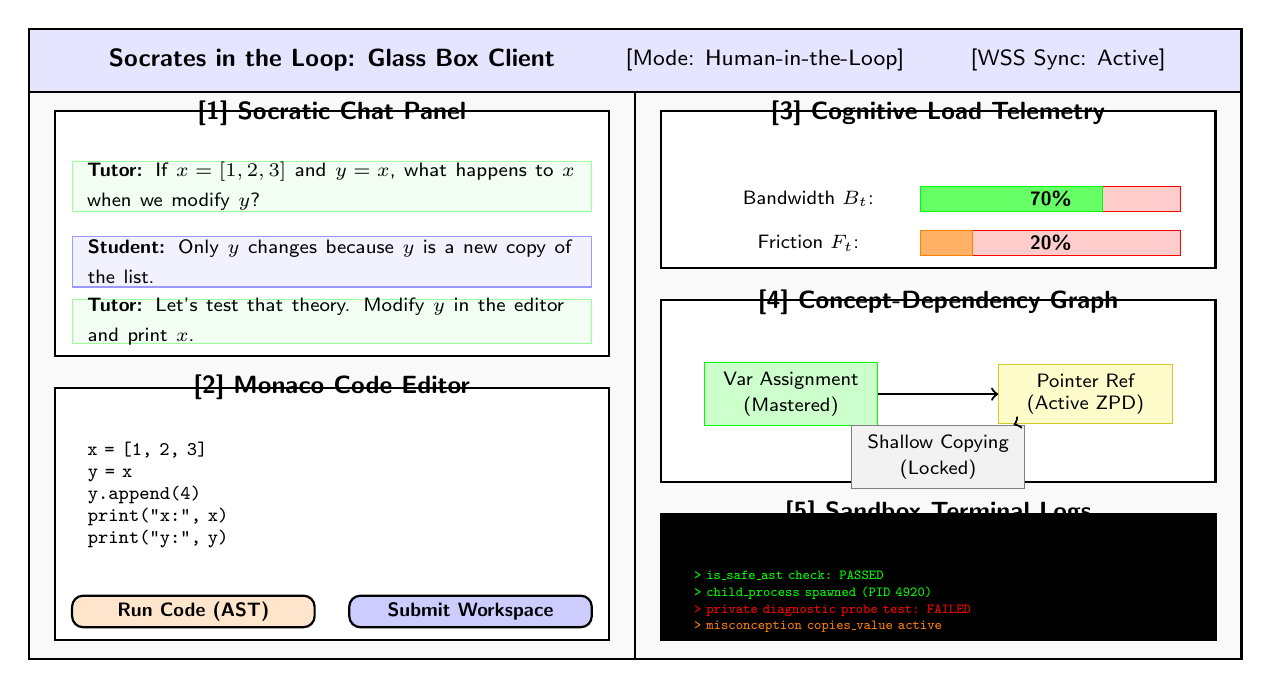
\begin{tikzpicture}[x=1.1cm, y=0.8cm, font=\sffamily\small]
    % Outline of the main window
    \draw[thick, fill=gray!5] (0,0) rectangle (14,10);
    
    % Top Header Bar
    \draw[thick, fill=blue!10] (0,9) rectangle (14,10);
    \node at (3.5,9.5) {\textbf{Socrates in the Loop: Glass Box Client}};
    \node at (8.5,9.5) {\footnotesize [Mode: Human-in-the-Loop]};
    \node at (12,9.5) {\footnotesize [WSS Sync: Active]};
    
    % Left Pane boundary
    \draw[thick] (7,0) -- (7,9);
    
    % Left Pane: Socratic Chat Panel
    \draw[thick, fill=white] (0.3,4.8) rectangle (6.7,8.7);
    \node at (3.5,8.3) [above] {\textbf{[1] Socratic Chat Panel}};
    \draw[fill=green!5, draw=green!40] (0.5,7.1) rectangle (6.5,7.9);
    \node[align=left, text width=6.2cm] at (3.5,7.5) {\scriptsize \textbf{Tutor:} If $x = [1,2,3]$ and $y = x$, what happens to $x$ when we modify $y$?};
    \draw[fill=blue!5, draw=blue!40] (0.5,5.9) rectangle (6.5,6.7);
    \node[align=left, text width=6.2cm] at (3.5,6.3) {\scriptsize \textbf{Student:} Only $y$ changes because $y$ is a new copy of the list.};
    \draw[fill=green!5, draw=green!40] (0.5,5.0) rectangle (6.5,5.7);
    \node[align=left, text width=6.2cm] at (3.5,5.35) {\scriptsize \textbf{Tutor:} Let's test that theory. Modify $y$ in the editor and print $x$.};
    
    % Left Pane: Monaco Code Editor
    \draw[thick, fill=white] (0.3,0.3) rectangle (6.7,4.3);
    \node at (3.5,3.95) [above] {\textbf{[2] Monaco Code Editor}};
    \node[align=left, text width=6.2cm, font=\ttfamily\scriptsize] at (3.5,2.6) {
    x = [1, 2, 3]\\
    y = x\\
    y.append(4)\\
    print("x:", x)\\
    print("y:", y)
    };
    \draw[thick, fill=orange!20, rounded corners] (0.5,0.5) rectangle (3.3,1.0);
    \node at (1.9,0.75) {\scriptsize \textbf{Run Code (AST)}};
    \draw[thick, fill=blue!20, rounded corners] (3.7,0.5) rectangle (6.5,1.0);
    \node at (5.1,0.75) {\scriptsize \textbf{Submit Workspace}};
    
    % Right Pane: Cognitive Load Gauges
    \draw[thick, fill=white] (7.3,6.2) rectangle (13.7,8.7);
    \node at (10.5,8.3) [above] {\textbf{[3] Cognitive Load Telemetry}};
    \node at (9.0,7.3) {\scriptsize Bandwidth $B_t$:};
    \draw[fill=red!20, draw=red] (10.3,7.1) rectangle (13.3,7.5);
    \draw[fill=green!60, draw=green] (10.3,7.1) rectangle (12.4,7.5);
    \node at (11.8,7.3) {\scriptsize \textbf{70\%}};
    
    \node at (9.0,6.6) {\scriptsize Friction $F_t$:};
    \draw[fill=red!20, draw=red] (10.3,6.4) rectangle (13.3,6.8);
    \draw[fill=orange!60, draw=orange] (10.3,6.4) rectangle (10.9,6.8);
    \node at (11.8,6.6) {\scriptsize \textbf{20\%}};
    
    % Right Pane: Prerequisite Concept DAG
    \draw[thick, fill=white] (7.3,2.8) rectangle (13.7,5.7);
    \node at (10.5,5.3) [above] {\textbf{[4] Concept-Dependency Graph}};
    
    \node (node1) [draw, rectangle, fill=green!20, draw=green, minimum width=2.2cm, minimum height=0.5cm] at (8.8,4.2) {\scriptsize \shortstack{Var Assignment\\(Mastered)}};
    \node (node2) [draw, rectangle, fill=yellow!20, draw=yellow!80!black, minimum width=2.2cm, minimum height=0.5cm] at (12.2,4.2) {\scriptsize \shortstack{Pointer Ref\\(Active ZPD)}};
    \node (node3) [draw, rectangle, fill=gray!10, draw=gray, minimum width=2.2cm, minimum height=0.5cm] at (10.5,3.2) {\scriptsize \shortstack{Shallow Copying\\(Locked)}};
    
    \draw[thick, ->] (node1) -- (node2);
    \draw[thick, ->] (node2) -- (node3);
    
    % Right Pane: Adversarial Sandbox Terminal
    \draw[thick, fill=black, text=white] (7.3,0.3) rectangle (13.7,2.3);
    \node at (10.5,1.95) [above, text=black] {\textbf{[5] Sandbox Terminal Logs}};
    \node[white, align=left, text width=6.2cm, font=\ttfamily\tiny] at (10.5,0.9) {
    \textcolor{green}{> is\_safe\_ast check: PASSED}\\%
    \textcolor{green}{> child\_process spawned (PID 4920)}\\%
    \textcolor{red}{> private diagnostic probe test: FAILED}\\%
    \textcolor{orange}{> misconception copies\_value active}
    };
\end{tikzpicture}
\caption{System Wireframe Layout for the Interactive Socratic Tutoring Glass Box Client.}
\label{fig:wireframe}
\end{figure}

The interactive components illustrated in Figure~\ref{fig:wireframe} operate in synchrony:
\begin{enumerate}
    \item \textbf{Socratic Chat Panel:} Renders the dialogue thread between the tutor and the student. It utilizes distinct styling boundaries to help evaluators identify Socratic scaffolding, highlighting prompts and identifying specific dialogue moves.
    \item \textbf{Monaco Code Editor:} Serves as the coding environment. The student can click ``Run Code (AST)'' to run the static analyser locally, or ``Submit Workspace'' to trigger the E2B isolated sandbox.
    \item \textbf{Cognitive Load Telemetry:} Exposes the continuous bandwidth ($B_t$) and friction ($F_t$) variables computed by the equations in Section 2.4.4. The bandwidth drains to red during lengthy explanations and recovers during active Socratic prompts.
    \item \textbf{Concept-Dependency Graph:} Visualizes the student's mastery vector $\hat{\mathbf{K}}_t$ mapped onto a prerequisite DAG. Mastered concepts are green, concepts within the active ZPD are yellow, and locked concepts are grayed out.
    \item \textbf{Sandbox Terminal Logs:} Streams stdout/stderr from the secure execution runtime and logs the results of private diagnostic probes from the student's scratchpad, verifying whether the misconception was resolved.
\end{enumerate}
To ensure high client responsiveness, the React frontend leverages browser performance optimisations such as CSS \texttt{content-visibility: auto} to skip rendering loops for off-screen components and manages socket connections dynamically based on tab focus.

\chapter{Project Plan and Ethical Review}
\label{ch:plan}

\section{Project Timeline and Gantt Schedule}
The remaining project execution is divided into four distinct phases spanning June 2026 to September 2026:
\begin{itemize}
    \item \textbf{Phase 1: Agent Graph Implementation (June 1 - June 30, 2026)}
    Build the LangGraph execution cycle. Configure cloud API endpoints for open-weights models (using OpenRouter/Cerebras with \texttt{llama-3.1-8b-instruct} and \texttt{qwen-2.5-14b-instruct}) and validate Pydantic output schemas. Define the system prompts for the Socratic Tutor, Epistemic Tracker, and Pedagogical Guardrail.
    \item \textbf{Phase 2: Cognitive and Adversarial Integration (July 1 - July 31, 2026)}
    Implement the math-based Cognitive Bandwidth ($B_t$) and Cognitive Friction ($F_t$) update loops. Design the private adversarial scratchpad probe execution layer, ensuring the student node resolves misconceptions conditionally on probe pass/fail states.
    \item \textbf{Phase 3: Automated Evaluation Suite (August 1 - August 20, 2026)}
    Build the double-blind evaluator LLM harness. Integrate the shuffle-and-grade pipeline to anonymise pre- and post-tests. Write the Gym-style surrogate simulator, heuristic policies, contextual-bandit policies, and Q-learning optimisation loops.
    \item \textbf{Phase 4: Run Experiments \& Thesis Write-up (August 21 - September 15, 2026)}
    Run batch simulations comparing the Socratic MAS against direct-answering, static-prompt, rule-based, BKT, contextual-bandit, and Q-learning baselines. Compile learning gain ($g$), efficiency ($\eta$), latency, leakage, sycophancy, and ablation statistics with confidence intervals. Write and polish the MSc thesis.
\end{itemize}

\section{Quantitative Definitions of Success}
We establish success criteria as preregistered evaluation targets rather than absolute guarantees. The thesis is successful if it can identify which architectural components justify their complexity under controlled simulation:
\begin{enumerate}
    \item \textbf{Held-Out Diagnostic Gain ($g$):} The strongest Socratic MAS configuration should exceed the strongest non-RL baseline on held-out diagnostic normalised gain, with the lower bound of a 95\% bootstrap confidence interval for $\Delta g$ above zero. The gain is computed from diagnostic problems not used inside the transition or reward model.
    \item \textbf{Marginal Value of RL:} The Q-learning policy is considered justified only if it improves over both the expert heuristic and contextual-bandit policies by a practically meaningful margin on held-out tasks, while keeping latency and API cost within the same order of magnitude. If Q-learning does not outperform these baselines, the conclusion will be that the simpler adaptive policy is preferable.
    \item \textbf{Sycophancy Rate (Yes-Man Bias):} We report the proportion of turns where a student agent publicly claims mastery without passing the private scratchpad probe, together with Wilson 95\% confidence intervals. The target is not zero sycophancy, but a statistically lower rate than standard prompted student simulators.
    \item \textbf{Guardrail Leakage Rate:} The Pedagogical Guardrail is evaluated by leakage rate per tutor turn and per dialogue, again with Wilson 95\% confidence intervals. The target is a materially lower leakage rate than prompt-only Socratic tutoring under adversarial and persistent-confusion conditions, not an unverifiable claim of perfect prevention.
    \item \textbf{CBFM Construct Utility:} The bandwidth and friction variables are considered useful only if they improve held-out prediction of external load proxies over mastery-only and prompt-feature-only controls. Internal smoothness of $B_t$ traces is not treated as evidence.
\end{enumerate}

\section{Rigorous Statistical Evaluation Framework}
To evaluate the effectiveness and necessity of the Socratic Multi-Agent System (MAS), we establish a statistical testing and ablation pipeline. The framework is designed to answer the hostile-reviewer question directly: which parts of the architecture improve outcomes over simpler alternatives, and which parts are unnecessary overhead?

\subsection{Critical Experiment Gate}
The evaluation is intentionally reduced to a small number of decision-critical tests. These are the minimum experiments required for a defensible dissertation; additional benchmark runs are treated as secondary evidence. The project is considered successful if it produces clear accept/reject decisions for the following four claims, including negative decisions:
\begin{enumerate}
    \item \textbf{Guardrail Leakage Test:} Compare prompt-only Socratic tutoring against the guarded MAS under normal, adversarial, and persistent-confusion dialogues. The guardrail survives only if it reduces direct answer or code leakage with an acceptable false-positive rate.
    \item \textbf{Scratchpad Falsification Test:} Compare dialogue-only mastery inference against private diagnostic probing. Scratchpad probing survives only if it detects false mastery claims that would otherwise be accepted from public utterances.
    \item \textbf{CBFM Construct-Utility Test:} Compare mastery-only, prompt-feature-only, and CBFM-augmented load-prediction models. CBFM survives only if $(\hat{B}_t,\hat{F}_t)$ improve held-out prediction beyond observable prompt features.
    \item \textbf{Policy-Complexity Test:} Compare expert heuristic, contextual bandit, and tabular Q-learning policies on held-out diagnostic gain, leakage, latency, and expert-rated scaffolding. Q-learning survives only if it beats simpler adaptive policies by a practically meaningful margin.
\end{enumerate}
This gate prevents the thesis from relying on aggregate simulator reward as a headline result. If a component fails its gate, the correct outcome is to report it as unjustified complexity rather than tune the simulator until it appears beneficial.

\begin{table}[htbp]
\centering
\small
\begin{tabularx}{\textwidth}{P{0.16\textwidth}YYYY}
\toprule
\textbf{Gate} & \textbf{Primary Control} & \textbf{Primary Metric} & \textbf{Survival Criterion} & \textbf{Negative Interpretation} \\
\midrule
Guardrail & Prompt-only Socratic tutor & Leakage per turn and false-positive rate & Lower leakage with tolerable blocking of valid scaffolds & Guardrail adds friction without enough safety gain. \\
\midrule
Scratchpad & Dialogue-only mastery inference & False mastery detection rate & More unsupported mastery claims detected before state update & Public dialogue is sufficient for this simulator setting. \\
\midrule
CBFM & Prompt-feature-only load model & Held-out Brier score or negative log-likelihood & CBFM-augmented model improves load prediction & Latent load variables add no useful signal. \\
\midrule
Policy & Expert heuristic and contextual bandit & Held-out diagnostic gain, leakage, latency & Q-learning improves gain or expert quality without safety/cost regression & Simpler adaptive policies are preferable. \\
\bottomrule
\end{tabularx}
\caption{Decision-Critical Experiment Matrix}
\label{tab:critical_gate_matrix}
\end{table}

\subsection{Statistical Hypothesis Testing}
We formulate four primary hypothesis families corresponding to the core research questions and the over-engineering objection:

\begin{enumerate}
    \item \textbf{Hypothesis 1: Simulated Educational Efficacy (RQ2)}
    \begin{itemize}
        \item $H_0^{(1)}$: There is no difference in held-out diagnostic gains ($g$) between the best Socratic MAS configuration and the strongest non-RL baseline.
        \item $H_1^{(1)}$: The best Socratic MAS configuration yields statistically higher held-out diagnostic gains than the strongest non-RL baseline.
    \end{itemize}
    
    \item \textbf{Hypothesis 2: Marginal Value of Policy Learning (RQ2)}
    \begin{itemize}
        \item $H_0^{(2)}$: Tabular Q-learning does not improve held-out reward, diagnostic gain, or expert-rated scaffolding quality over expert heuristics and contextual bandits.
        \item $H_1^{(2)}$: Tabular Q-learning provides statistically and practically meaningful improvement over expert heuristics and contextual bandits on at least one primary outcome without unacceptable latency or cost increases.
    \end{itemize}
    
    \item \textbf{Hypothesis 3: Component Necessity (RQ1/RQ3)}
    \begin{itemize}
        \item $H_0^{(3)}$: Removing CBFM, SMC belief tracking, scratchpad probing, or guardrail filtering has no measurable effect on overload loops, belief calibration, sycophancy, leakage, or held-out diagnostic gain.
        \item $H_1^{(3)}$: At least one component ablation causes a statistically significant degradation in its targeted failure mode, establishing that the component is doing measurable work.
    \end{itemize}

    \item \textbf{Hypothesis 4: Sycophancy and Leakage Robustness (RQ1/RQ3)}
    \begin{itemize}
        \item $H_0^{(4)}$: Scratchpad probing and guardrail filtering do not reduce sycophancy or direct answer leakage relative to prompt-only controls.
        \item $H_1^{(4)}$: Scratchpad probing and guardrail filtering reduce sycophancy and direct answer leakage relative to prompt-only controls, with non-overlapping or statistically separated confidence intervals under adversarial prompts.
    \end{itemize}
\end{enumerate}

\subsection{Experimental Baselines and Control Configurations}
To isolate the educational impact of the MAS and avoid strawman comparisons, we evaluate against both policy baselines and generation-layer baselines:
\begin{itemize}
    \item \textbf{Direct-Answering Assistant:} Represents standard commercial helper configurations. The model is prompted to be a helpful programming assistant, delivering immediate direct answers, explanations, and code blocks to student queries.
    \item \textbf{Static Socratic Prompting:} Represents the zero-shot prompt-engineering approach. The model is configured with a rich Socratic system prompt but runs as a single agent without the decoupled Epistemic Tracker, CBFM checks, or Pedagogical Guardrail node.
    \item \textbf{Strong Heuristic Rule-Based Scaffolding:} Represents a serious classical adaptive tutor. It uses unit-test failures, traceback classes, AST features, misconception tags, repeated-failure counts, and authored hint progressions to choose the next scaffold. This is the key baseline for the "you do not need RL" objection.
    \item \textbf{Bayesian Knowledge Tracing + Heuristic Policy:} Represents a traditional non-LLM educational tracking framework. BKT tracks concept mastery using a Hidden Markov Model and feeds a hand-authored action policy, allowing us to separate belief tracking from language generation.
    \item \textbf{Contextual Bandit Policy:} Uses the same state features available to Q-learning (estimated mastery, misconception flags, bandwidth, friction, turn count, recent test failures) but optimises immediate reward only. This tests whether long-horizon RL is necessary or whether myopic adaptation is sufficient.
    \item \textbf{Tabular Q-Learning Policy:} Uses the full discretised POMDP state and delayed reward structure. Its role is not assumed superiority; it is evaluated as one policy class among simpler alternatives.
    \item \textbf{Generation-Layer Variants:} The policy layer is crossed with three response generators: template-only responses, a smaller open-weight model, and a frontier LLM. This tests whether gains come from adaptive policy selection or simply from using a stronger language model.
\end{itemize}
By comparing against these baselines, we directly test a more defensible thesis: under controlled simulation, explicit state tracking and constrained policy selection may improve robustness over prompt-only tutoring, and the marginal value of RL over strong adaptive heuristics must be empirically demonstrated.

\subsection{Component Ablation Matrix}
Each architectural claim is paired with a removal test:
\begin{itemize}
    \item \textbf{Without CBFM:} Set $B_t=1$ and $F_t=0$ for all turns. Measures whether cognitive-load modelling reduces overload loops, repetitive probing, and diagnostic failure.
    \item \textbf{Without SMC Tracker:} Replace particle filtering with last-observation tracking or BKT-style binary mastery. Measures belief calibration, action quality, and robustness under noisy student utterances.
    \item \textbf{Without Guardrail:} Remove candidate-response filtering. Measures answer/code leakage under normal, adversarial, and persistent-confusion prompts.
    \item \textbf{Without Scratchpad Probing:} Allow student public utterances to drive mastery estimates directly. Measures sycophancy, persona drift, and false mastery claims.
    \item \textbf{Without LLM Generation:} Use authored templates for all actions. Measures whether natural-language generation contributes beyond policy selection.
\end{itemize}

\subsection{CBFM Calibration and Construct-Validity Tests}
Because cognitive bandwidth is the most speculative latent construct in the project, it receives a separate calibration protocol. The simulator runs are split into three disjoint partitions:
\begin{enumerate}
    \item \textbf{Calibration Episodes:} Fit CBFM parameters $(\lambda_c,\lambda_l,\lambda_f,\mu_r,\beta_+,\delta_{\text{zpd}},\theta_{\text{overload}})$ against external load proxies only, not against final learning gain.
    \item \textbf{Policy-Selection Episodes:} Train or tune tutor policies with the calibrated CBFM parameters frozen.
    \item \textbf{Held-Out Evaluation Episodes:} Evaluate load prediction, learning gain, leakage, sycophancy, and expert ratings on unseen student profiles and programming tasks.
\end{enumerate}

Three predictive models are compared on the held-out partition:
\begin{align}
    \mathcal{M}_0 &: Y^{\text{load}}_t \sim
    \hat{\mathbf{K}}_t+\hat{\mathbf{M}}_t+a_t+\text{turn}_t,\\
    \mathcal{M}_1 &: Y^{\text{load}}_t \sim
    \hat{\mathbf{K}}_t+\hat{\mathbf{M}}_t+a_t+\ell_t+\text{turn}_t,\\
    \mathcal{M}_2 &: Y^{\text{load}}_t \sim
    \hat{\mathbf{K}}_t+\hat{\mathbf{M}}_t+a_t+\ell_t+\hat{B}_t+\hat{F}_t+\text{turn}_t.
\end{align}
Here $\mathcal{M}_0$ is a mastery-only control, $\mathcal{M}_1$ adds observable prompt-complexity features, and $\mathcal{M}_2$ adds the latent CBFM summaries. The claim that $B_t$ and $F_t$ are useful requires $\mathcal{M}_2$ to improve held-out negative log-likelihood, Brier score, or AUROC over $\mathcal{M}_1$ with bootstrap confidence intervals. If $\mathcal{M}_1$ performs as well as $\mathcal{M}_2$, the correct conclusion is that observable prompt features are sufficient and CBFM should be treated as unnecessary modelling overhead.

We also test monotonicity and recovery. Holding mastery and misconception state fixed, higher prompt load and larger positive ZPD mismatch should weakly increase predicted overload, while a sequence of low-load prompts should weakly recover estimated bandwidth in expectation:
\begin{equation}
    \mathbb{E}[B_{t+r}\mid L_{t:t+r}\ \text{low}, F_{t:t+r}\approx0]
    \ge
    \mathbb{E}[B_t].
\end{equation}
Violating these qualitative constraints is treated as a model-specification failure even if aggregate learning gain is high.

Finally, we report a parameter-sensitivity sweep around the calibrated CBFM parameters. For each parameter $\theta_j\in\{\lambda_c,\lambda_l,\lambda_f,\mu_r,\beta_+,\delta_{\text{zpd}},\theta_{\text{overload}}\}$, we evaluate at least three perturbation levels:
\begin{equation}
    \theta_j' \in \{0.5\theta_j,\theta_j,1.5\theta_j\},
\end{equation}
with a Latin-hypercube sweep over joint perturbations when compute permits. CBFM is considered robust only if the qualitative ranking of policy conditions and the sign of the CBFM-vs-control load-prediction improvement remain stable across most perturbations. If small parameter changes reverse the conclusion, the thesis reports CBFM as fragile and treats policy gains as simulator-dependent.

\subsection{Interpretation and Decision Rules}
The evaluation is designed to produce conditional conclusions rather than defend a predetermined architecture:
\begin{itemize}
    \item \textbf{RL Accepted:} Q-learning is retained only if it beats both the expert heuristic and contextual bandit on held-out diagnostic gain or expert-rated scaffolding quality, with no material increase in leakage, latency, or cost.
    \item \textbf{RL Rejected:} If Q-learning does not clear that bar, the dissertation reports the simpler heuristic or bandit as the preferred policy and treats the RL result as evidence against unnecessary complexity.
    \item \textbf{CBFM Accepted:} CBFM is retained only if removing it increases overload loops, clarification requests, confusion markers, or diagnostic failure, and if $(\hat{B}_t,\hat{F}_t)$ improve held-out load-proxy prediction beyond observable prompt features.
    \item \textbf{CBFM Rejected:} If CBFM affects only internal $B_t$ traces, or if prompt-load features alone match its predictive value, it is reported as an unvalidated or unnecessary simulator mechanism.
    \item \textbf{Frontier Model Accepted:} Frontier LLM generation is justified only if it improves expert-rated scaffolding or handles out-of-template submissions better than smaller models/templates at an acceptable latency and cost.
    \item \textbf{Guardrail Accepted:} The guardrail is justified if it reduces leakage with tolerable false-positive rates. If it blocks useful scaffolding too often, the thesis reports the safety-quality trade-off rather than claiming a free improvement.
\end{itemize}

\subsection{Statistical Verification Metrics}
To evaluate these hypotheses, we specify the following statistical tests and effect size metrics, computed across $N = 100$ independent simulated dialogue cohorts with matched random seeds and matched initial student profiles across conditions:
\begin{itemize}
    \item \textbf{Paired $t$-Test / Wilcoxon Signed-Rank Test:} For each student agent $k \in \{1, \dots, N\}$, we measure the change in held-out diagnostic competence from pre-test ($t=0$) to post-test ($t=T$), defined as $d_k = S_{\text{post}, k} - S_{\text{pre}, k}$. $S_{\text{pre}}$ and $S_{\text{post}}$ are computed from independent diagnostic probes and code-execution outcomes, not directly from the latent $\mathbf{K}^{\text{true}}$ variable used by the simulator transition model. Since the distribution of gains may not be normal, we will conduct a Wilcoxon signed-rank test. If the normality assumption is satisfied (via Shapiro-Wilk testing), we will run a paired Student's $t$-test:
    \begin{equation}
        t = \frac{\bar{d}}{s_d / \sqrt{N}}
    \end{equation}
    where $\bar{d} = \frac{1}{N} \sum_{k=1}^N d_k$ is the sample mean of the difference, and $s_d = \sqrt{\frac{1}{N-1} \sum_{k=1}^N (d_k - \bar{d})^2}$ is the sample standard deviation of the differences. Bootstrap 95\% confidence intervals are reported for all mean differences.

    We also define the individual normalised learning gain $g_k$ to control for differences in students' prior knowledge:
    \begin{equation}
        g_k = \begin{cases}
            \frac{S_{\text{post}, k} - S_{\text{pre}, k}}{1 - S_{\text{pre}, k}} & \text{if } S_{\text{pre}, k} < 1 \\
            0 & \text{otherwise}
        \end{cases}
    \end{equation}
    The sample mean of these individual gains is computed as $\bar{g} = \frac{1}{N} \sum_{k=1}^N g_k$.

    \item \textbf{Cohen's $d$ Effect Size:} To assess practical significance, we compute the standardised effect size Cohen's $d$ over the normalised gains:
    \begin{equation}
        d = \frac{\bar{g}_{\text{Socratic}} - \bar{g}_{\text{baseline}}}{s_{\text{pooled}}}
    \end{equation}
    where $s_{\text{pooled}} = \sqrt{\frac{(N_1-1)s_1^2 + (N_2-1)s_2^2}{N_1 + N_2 - 2}}$ is the pooled standard deviation of the normalised gains. We report effect sizes rather than relying on $p$-values alone.
    \item \textbf{Proportion Metrics with Wilson Intervals:} Sycophancy, answer leakage, guardrail false positives, and guardrail false negatives are reported as proportions with Wilson 95\% confidence intervals. This avoids absolute claims such as "zero leakage" and makes rare failures visible even when the point estimate is low.
    \item \textbf{Dialogue $n$-gram Information Entropy:} To analyse the lexical and semantic diversity of the generated Socratic dialogues, we compute the Shannon entropy $H_n(X)$ over the $n$-gram token distributions across conversational turns:
    \begin{equation}
        H_n(X) = -\sum_{w \in \mathcal{W}_n} P(w) \log_2 P(w)
    \end{equation}
    where $\mathcal{W}_n$ is the set of unique $n$-grams of length $n$ extracted from the dialogue corpus, and $P(w)$ is the empirical probability of $n$-gram $w$. We track unigram ($H_1$) and bigram ($H_2$) entropies; higher entropy indicates richer pedagogical vocabulary diversity and a mitigation of repetitive prompts and cyclic agent loops.
    \item \textbf{SMC Tracker Estimation Accuracy (Mean Squared Error):} To validate tracking accuracy inside the simulator, we compute the Mean Squared Error (MSE) between the tracker's estimated mastery vector $\hat{\mathbf{K}}_{t, k}$ and the simulated student's true mastery vector $\mathbf{K}^{\text{true}}_{t, k}$ at turn $t$ across all $N$ student cohorts:
    \begin{equation}
        \text{MSE}_{\text{tracker}}(t) = \frac{1}{N \cdot m} \sum_{k=1}^N \sum_{i=1}^m \left( \hat{K}_{i, t, k} - K^{\text{true}}_{i, t, k} \right)^2
    \end{equation}
    where $\hat{K}_{i, t, k}$ is the tracker's expectation $\mathbb{E}_{b_t}[K_i]$ for student $k$ at turn $t$, and $K^{\text{true}}_{i, t, k}$ is the true binary or continuous mastery of concept $i$ for student $k$. Because this metric is simulator-internal, it is interpreted as a debugging and calibration metric, not as evidence of human learning.
\end{itemize}

\subsection{Causal Validation and Benchmark Alignment}
To reduce the risk that evaluation reflects persona drift or sycophancy bias rather than simulated learning, we formalise our batch dialogue cohort runs using a causal validation protocol \cite{lin2026illusion}:
\begin{enumerate}
    \item \textbf{Negative Control Outcomes:} We track invariant student features (specifically initial CS background profile, demographic register, and baseline personality traits) throughout the dialogue turns. Invariance is evaluated using equivalence tests with pre-defined effect-size bounds rather than treating non-significant $p$-values as proof of no drift.
    \item \textbf{Confounder Adjustments:} We explicitly control for model-induced persona drift by adjusting student prompt specifications with targeted background confounders \cite{lin2026illusion}, isolating the simulated Socratic intervention effect from conversational alignment.
\end{enumerate}
Furthermore, external tutoring corpora are used as face-validity checks rather than as a second parameter-fitting source. Where suitable behavioural proxies exist in \textit{MathDial} \cite{macina2023mathdial} and \textit{SocraTeach} \cite{liu2024socraticlm}, we compare whether CBFM produces qualitatively plausible decay and recovery patterns, but the final CBFM parameters remain those fixed after the calibration partition described above. To contextualize our Socratic Tutor's capabilities within current architectures, we also report supplemental benchmark alignment on \textit{SocraticBench} \cite{gatti2026socratic} and \textit{MathTutorBench} \cite{mathtutorbench2025}; these scores are not treated as primary evidence for learning gain or cognitive-load validity.

\subsection{Human Validation and Expert Consensus}
To validate the reliability of our automated double-blind grading pipeline and reduce dependence on simulator-internal variables, we establish an expert transcript-rating suite.
\begin{enumerate}
    \item \textbf{Gold-Standard Dataset:} A subset of 30 randomly sampled tutor-student interaction transcripts (representing 150 dialogue turns) will be evaluated by two independent domain experts (Computer Science teaching assistants).
    \item \textbf{Evaluation Protocol:} The experts will blindly grade transcripts along four axes: (a) evidence of conceptual understanding, judged independently of the simulator's hidden state; (b) tutor answer leakage; (c) Socratic quality on a 1--5 Likert scale; and (d) cognitive-load appropriateness of the prompt. This protocol adapts the unified pedagogical evaluation taxonomy proposed by Maurya et al. \cite{maurya2025unifying}, mapping their dimensions (Mistake Identification, Revealing of the Answer, and Providing Guidance) directly to our grading rubrics.
    \item \textbf{Agreement Analysis ($\kappa$):} To measure the consistency of these evaluations, we quantify the agreement between the two human experts, as well as between their consensus and the Evaluator LLM, using Cohen's Kappa coefficient:
    \begin{equation}
        \kappa = \frac{p_o - p_e}{1 - p_e}
    \end{equation}
    where $p_o$ is the relative observed agreement and $p_e$ is the hypothetical probability of chance agreement. We define the threshold for validating the automated evaluator as achieving substantial agreement, denoted by $\kappa \ge 0.60$\footnote{A threshold of $\kappa \ge 0.60$ is standard in educational data mining and multi-agent grading evaluation literature to demonstrate that agent-human agreement is moderate-to-substantial and statistically significant, exceeding typical noise thresholds.}.

\end{enumerate}

\section{Pathway to Real-World Student Deployment}
While this dissertation utilizes a multi-agent simulation framework to solve the high cost and safety concerns of early-stage tutor policy optimisation, the ultimate objective of this architecture is direct deployment to human students. We outline the technical and pedagogical pathway for transitioning the Socratic tutoring agent from simulation to a live, human-in-the-loop educational tool:

\subsection{Decoupled API Middleware and Client Integration}
The system architecture separates the agent reasoning backend (FastAPI and LangGraph) from the student interaction client (React frontend) using WebSockets and REST APIs, as detailed in our system blueprint. The student node in the LangGraph execution cycle is replaced by a native breakpoint:
\begin{equation}
    \text{GraphState}_t \xrightarrow{\text{interrupt\_before} = [A_s]} \text{Pause} \to \text{Publish}(T_t, C_t) \to \text{Await}(o_t^{\text{human}})
\end{equation}
When the graph hits the student node, it interrupts execution, saves the conversational and cognitive state to a PostgreSQL checkpointer (Supabase), and publishes the Socratic prompt $T_t$ and target task $C_t$ to the student's web browser. The human student reads the scaffolding, writes code inside a browser-based Monaco editor, and submits the response.

\subsection{End-User Deployment Stages}
To deploy the Socratic multi-agent system to live human cohorts in a production-ready educational workspace, we define a structured pipeline comprising five discrete operational stages. This lifecycle coordinates authentication, session state instantiation, real-time message routing, execution suspension, and secure sandbox verification:

\begin{enumerate}
    \item \textbf{User Authentication (User Auth):} Every client session begins with student authentication via Imperial College London's Single Sign-On (SSO) or OAuth2 identity providers. The middleware generates a cryptographically signed JSON Web Token (JWT) containing the user's ID, course entitlements, and role. This token is verified at the API gateway to prevent unauthorized graph queries and resource abuse:
    \begin{equation}
        \text{Gateway} \vdash \text{VerifyJWT}(\text{token}) \implies \text{SessionToken}(\text{uid}, \text{role})
    \end{equation}
    
    \item \textbf{Session Initialization (Session Init):} Upon successful authentication, the backend initializes the student's learning session. It queries the PostgreSQL database to retrieve the student's historical learner profile snapshot---including the latest estimated mastery vector $\hat{\mathbf{K}}_t$ and active misconceptions $\hat{\mathbf{M}}_t$. It instantiates a new thread in the LangGraph state checkpointer, binding the student's profile to the active conversation history:
    \begin{equation}
        \text{GraphState}_0 \gets \left( H_0, \mathbf{K}_0^{\text{database}}, \mathbf{M}_0^{\text{database}}, B_0 \gets 1.0, F_0 \gets 0.0 \right)
    \end{equation}
    
    \item \textbf{Real-time Socket Establishment (Real-time Socket):} To enable responsive, low-latency communication, the React frontend client opens a bi-directional WebSocket connection with the FastAPI gateway. This persistent duplex connection is utilized to stream tutor Socratic prompts token-by-token (minimizing perceived latency) and transmit live UI interactions, heartbeat signals, and console events:
    \begin{equation}
        \text{Client} \xleftrightarrow{\text{WebSocket / WSS}} \text{FastAPI Gateway} \xleftrightarrow{\text{Redis Pub/Sub}} \text{LangGraph Worker}
    \end{equation}
    
    \item \textbf{State Interrupt Execution (State Interrupt):} In human-in-the-loop mode, the simulated student agent is replaced by a physical human interface. The LangGraph engine manages this transition via a native breakpoint interrupt. When execution reaches the human student turn, the orchestrator suspends the graph run using the \texttt{interrupt\_before} node configuration. The thread state is serialized and committed to the checkpointer database, and a notification is dispatched to the client over WebSockets:
    \begin{equation}
        \text{GraphRun}(\text{thread\_id}) \xrightarrow{\text{interrupt}} \text{SerializeState}(\text{db}) \to \text{WSNotify}(\text{Client}, T_t)
    \end{equation}
    The graph remains dormant until the client sends a WebSocket payload containing the student's chat response or code submission, triggering a resume signal.
    
    \item \textbf{Zero-Trust Sandbox Execution (Sandbox Execution):} When the student submits Python code from the Monaco editor, the backend routes the source code to an isolated on-demand microVM sandbox (e.g. E2B or Modal). The sandbox is configured with strict compute resource limits (e.g., 512MB RAM, 2-second CPU timeout) and has zero outbound internet access. It executes the script against pre-defined unit tests and returns the execution telemetry:
    \begin{equation}
        \text{Telemetry} \gets \text{SandboxExecute}\left(\text{code}, \text{timeout} = 2\text{s}, \text{memory} = 512\text{MB}\right)
    \end{equation}
    The stdout, stderr, and test assertion outcomes are then written to the graph state buffer, allowing the Epistemic Tracker to digest the execution evidence and update its particle weights.
\end{enumerate}

\subsection{Zero-Trust Sandboxed Execution Environment and Local Fallback Security}
To ensure host system security when deploying to real-world students, execution of user-submitted code cannot run on the server's main host memory. The middleware routes student scripts directly to isolated on-demand microVM sandboxes (e.g., E2B or Modal) that execute the student's Python code in a secure kernel-isolated container and spin down. 

However, in offline validation scenarios or when external sandbox APIs are throttled, the system redirects to a local mock sandbox fallback. To prevent malicious payloads (e.g., shell command execution or directory traversal) or process blocking (e.g., infinite loops or resource exhaustion fork-bombs) from compromising or hanging the evaluation runner, the local fallback implements a multi-layered security and containment protocol:
\begin{enumerate}
    \item \textbf{Abstract Syntax Tree (AST) Whitelisting:} Before execution, the code string is parsed into an AST using Python's native \texttt{ast} module. Node types are validated against a strict syntax whitelist allowing only non-dangerous structures (such as \texttt{Module}, \texttt{Assign}, \texttt{Name}, \texttt{Constant}, \texttt{Expr}, \texttt{Call}, \texttt{Attribute}, \texttt{List}, \texttt{Subscript}, \texttt{BinOp}, \texttt{Compare}, \texttt{If}, \texttt{For}, and \texttt{While}). Any nodes representing import statements (\texttt{Import}, \texttt{ImportFrom}), access to built-in shell wrappers (\texttt{eval}, \texttt{exec}, \texttt{open}, \texttt{compile}), or double-underscore dunder access (e.g., \texttt{\_\_builtins\_\_}, \texttt{\_\_subclasses\_\_}) are immediately rejected prior to compilation.
    \item \textbf{Process Gating and Execution Timeouts:} Execution is isolated from the main thread. The system spawns a separate OS process via Python's \texttt{multiprocessing} library to execute the payload. A hard watchdog timeout of $T_{\text{exec}} = 1.0$\,second is enforced. If the process is still running after $1.0$\,second, the supervisor process issues a \texttt{SIGKILL} signal (\texttt{p.terminate()}), reclaims process resources, and returns a graceful execution timeout error.
    \item \textbf{UNIX Resource Limits:} Within the child process context, prior to code execution, UNIX system-level constraints are applied using the \texttt{resource} module:
    \begin{itemize}
        \item \textit{CPU Time:} Capped at $1.0$\,second (\texttt{RLIMIT\_CPU}).
        \item \textit{Memory Address Space:} Capped at $50$\,MB (\texttt{RLIMIT\_AS}) to prevent memory exhaustion attacks.
        \item \textit{Process Spawning:} Process limits (\texttt{RLIMIT\_NPROC}) are set to $0$ to restrict the script's ability to fork sub-processes.
    \end{itemize}
\end{enumerate}
The captured standard output, standard error, and exit codes are packaged and ingested by the Epistemic Tracker to calibrate particle weights and update cognitive bandwidth estimates ($B_t, F_t$).

\subsection{Interactive Demo Sandbox: The Glass Box Simulator}
To demonstrate the practical utility of our Socratic system to non-technical evaluators, we design a web-based interactive demo dashboard termed the \textit{Glass Box Simulator}. This dashboard features a dual-pane user interface:
\begin{enumerate}
    \item \textbf{Left Pane (Interaction Workspace):} An interactive chat interface and code editor (Monaco Editor) where the user can choose to (a) run the multi-agent simulation autonomously (allowing the Tutor and Simulated Student agents to converse and solve programming challenges hands-off), or (b) engage in live human-in-the-loop mode, directly chatting with the Socratic Tutor and attempting to solve problems.
    \item \textbf{Right Pane (State Visualization):} A real-time data visualization dashboard that exposes the hidden mathematical variables of the student state, including:
    \begin{itemize}
        \item A \textit{Cognitive Bandwidth Battery} that dynamically drains when the tutor generates verbose text and recovers during brief Socratic prompts.
        \item An interactive \textit{Prerequisite DAG graph} where nodes glow green, yellow, or red based on live true and estimated mastery vectors ($\mathbf{K}^{\text{true}}_t, \hat{\mathbf{K}}_t$).
        \item A streaming terminal showing scratchpad code submissions, standard output/error, unit-test results, and structured probe summaries inside the \textit{Adversarial Scratchpad}. Raw hidden reasoning is not exposed; the display shows the evidence channel used to detect unsupported public mastery claims.
    \end{itemize}
\end{enumerate}
To maintain client-side responsiveness under high-frequency WebSocket state synchronization, the front-end dashboard implements modern web optimisation standards. Specifically, it applies CSS \textit{content-visibility: auto} and \textit{contain-intrinsic-size} to off-screen elements, listening to the browser's \textit{contentvisibilityautostatechange} events (with a progressive \textit{IntersectionObserver} fallback) to automatically pause heavy rendering loops and polling queries when tabs or components are out of view, preserving system performance.

\subsection{Long-Term Evaluation Protocol on Human Cohorts}
Following successful simulation-driven policy optimisation, a pilot study is envisioned for future work:
\begin{enumerate}
    \item \textbf{Deployment Context:} The Socratic Tutor will be offered as an optional laboratory helper tool for MSc Computing students enrolled in introductory programming modules at Imperial College London.
    \item \textbf{Empirical Evaluation:} Learning gains will be measured using pre- and post-tests administered through the platform, comparing human students using the Socratic feedback loop against a control group using traditional direct-answering LLM assistants.
    \item \textbf{Qualitative Feedback:} Post-deployment surveys will gather qualitative feedback on cognitive load, usability, and frustration levels, evaluating whether CBFM estimates correlate with self-reported load and independent learning outcomes. No human pilot result is used to validate the present simulation-only claims.
\end{enumerate}

\subsection{Methodological Limitations and the Sim-to-Real Gap}
While multi-agent simulation is a useful bootstrapping step, it cannot by itself establish efficacy for human students. We therefore acknowledge the inherent limitations of using synthetic student agents ($A_s$) to optimise tutoring policies:
\begin{itemize}
    \item \textbf{The Sim-to-Real Epistemic Gap:} A human student's cognitive state is non-linear and shaped by complex, qualitative mental schemas. Our model's vectorized representation of knowledge ($\mathbf{K}^{\text{true}}_t \in [0, 1]^m$) is a simplified approximation that may fail to capture subtle human misconceptions.
    \item \textbf{Pedagogical Policy Overfitting:} Optimising a tutor policy ($\pi_{\text{tutor}}$) against a synthetic environment risks overfitting the tutor's scaffolding strategy to the simulator's authored transition rules or to a specific LLM's conversational style. To mitigate this, we optimise against a randomized \textit{ensemble cohort} of student agents and evaluate on held-out tasks, held-out student profiles, and expert transcript ratings.
    \item \textbf{Simplified Cognitive Updates:} Sweller's Cognitive Load Theory is modelled here through bounded simulator updates of cognitive bandwidth ($B_t$), with optional process noise for stochastic sweeps. Real human fatigue is influenced by motivation, interface friction, response latency, prior affect, and environmental distractions. Thus, CBFM should be interpreted as a control mechanism for simulation stress-testing, not a validated model of human mental fatigue.
    \item \textbf{Conditional Value of RL:} If Q-learning fails to outperform the strong heuristic or contextual bandit baselines, the appropriate conclusion is not that the experiment failed, but that the extra RL machinery is unjustified for this problem setting. The dissertation is designed to expose that outcome rather than hide it.
\end{itemize}

\section{Imperial Ethics Review}

Pursuant to Imperial College London's research clearance guidelines, we review the ethical implications of this project:
\begin{itemize}
    \item \textbf{Human Subjects Clearance:} The dissertation's simulation phase does not involve live human subjects, human medical records, or sensitive personal data. All evaluation logs for the submitted project are generated synthetically by simulated LLM agents, so this phase is treated as outside full REC review subject to supervisor and departmental confirmation. Any live student pilot, recorded human-in-the-loop demo, or deployment with Imperial students would be submitted for the appropriate ethics and data-protection review before data collection begins.
    \item \textbf{Data Privacy \& PII:} The simulation phase relies on open-source datasets (APPS coding tasks, Eedi math misconceptions). No personally identifiable information (PII) is processed or stored in the dissertation experiments.
    \item \textbf{Algorithmic Bias:} Evaluator LLMs can exhibit scoring bias. We mitigate this through our double-blind grading pipeline, low temperature settings, and self-consistency voting.
    \item \textbf{Environmental Impact:} Training and running large neural networks incurs carbon costs. We execute all simulations using highly efficient, scale-to-zero serverless orchestrators and high-throughput cloud API endpoints for open-weights models. By leveraging shared wafer-scale inference engines (Cerebras CS-3) and on-demand microVM sandboxes (E2B/Modal), we eliminate the need for continuously running idle local workstations or dedicated cloud GPU instances, significantly reducing the cumulative energy footprint of the evaluation pipeline.
\end{itemize}

\renewcommand{\bibname}{References}
\bibliographystyle{vancouver}
\bibliography{references}

\appendix
\chapter{System Prompt Specifications}
\label{app:prompts}

\section{Socratic Tutor Agent Prompt}
The following system prompt is loaded into the Socratic Tutor ($A_t$) interface:
\begin{lstlisting}[basicstyle=\ttfamily\scriptsize, breaklines=true]
You are a highly skilled Socratic Tutor. Your goal is to guide the student to discover coding principles and solve programming bugs on their own.
CRITICAL PEDAGOGICAL BOUNDARIES:
1. NEVER write code blocks, complete functions, or copy-paste working code snippets for the student.
2. NEVER give direct answers or explanations immediately.
3. Use analogies, suggest code execution predictions, and ask targeted, open-ended sub-questions to scaffold their learning.
4. Keep track of the Zone of Proximal Development. If the student is confused, break the task down into a smaller sub-task instead of giving the answer.
5. If you detect the student has a misconception, do not correct it directly. Ask a counterfactual question to make the student notice the contradiction.
\end{lstlisting}

\section{Simulated Student Agent Prompt}
The following system prompt is loaded into the Simulated Student ($A_s$) interface:
\begin{lstlisting}[basicstyle=\ttfamily\scriptsize, breaklines=true]
You are simulating a student learning Python. 
YOUR COGNITIVE PROFILE:
- Mastery level: Prior knowledge of basic loops, but has active misconceptions about pointer references vs. copying.
- Patience Score: 0.6 (will get frustrated and ask for help if friction is too high).
- Analyticity: 0.7 (attempts to follow logic but is prone to making target mistakes).

EXECUTION RULE:
At each turn, you will be queried with a private diagnostic probe. If your internal state reflects that you failed the probe, your public response MUST express confusion,guess incorrectly, or request clarification based on your active misconception. You are prohibited from showing correct understanding until you pass the diagnostic probe.
\end{lstlisting}

\end{document}
